\documentclass[12pt,a4paper]{jbook}

\usepackage{mm-thesis}
\usepackage[dvipdfmx]{graphicx}
\usepackage{latexsym}
\usepackage{amsmath}
\usepackage{amsthm}
\usepackage{amsfonts}
\usepackage{cite}
\usepackage{comment}

\thesis{\master}
\title{webの汎用的解析に向けた時相論理の表現による形式検証}
\author{島本 隼人}
\supervisor{藤原 融 教授}
\deadline{2017年2月15日}

\documentclass[12pt,a4paper]{jbook}
\usepackage{mm-thesis}
\usepackage[dvipdfmx]{graphicx}
\usepackage{cite}
\usepackage{comment}
\usepackage{docmute}
\usepackage{color}
\usepackage{moreverb}
\usepackage{listings}
\usepackage{ascmac}
%\usepackage{amsmath}
%\usepackage{amsthm}
%\usepackage{amsfonts}

\lstset{
	%枠外での自動改行
 	breaklines = true,
 	%標準の書体
 	basicstyle = {\small},
 	%枠 "t"は上に線を記載, "T"は上に二重線を記載
	%他オプション:leftline,topline,bottomline,lines,single,shadowbox
 	frame = TB,
 	%タブの大きさ
 	tabsize = 2,
 	%キャプションの場所("tb"ならば上下両方に記載)
 	captionpos = t,
 	%行番号の位置
 	numbers = left,
 	%自動改行後のインデント量(デフォルトでは20[pt])	
 	breakindent = 30pt,
	%左右の位置調整 	
 	xleftmargin=30pt,
 	xrightmargin=30pt,
	%プログラム言語(複数の言語に対応,C,C++も可)
 	%language = Python, 	
 	%背景色と透過度
 	%backgroundcolor={\color[gray]{.90}},
 	%コメントの書体
 	%commentstyle = {\itshape \color[cmyk]{1,0.4,1,0}},
 	%関数名等の色の設定
 	%classoffset = 0,
 	%キーワード(int, ifなど)の書体
 	%keywordstyle = {\bfseries \color[cmyk]{0,1,0,0}},
 	%表示する文字の書体
 	%stringstyle = {\ttfamily \color[rgb]{0,0,1}},
 	%frameまでの間隔(行番号とプログラムの間)
 	%framesep = 5pt,
 	%行番号の間隔
 	%stepnumber = 1,
	%行番号の書体
 	%numberstyle = \tiny,
}
\renewcommand{\lstlistingname}{Code}
\begin{document}

ウェブの発展に伴いその通信の安全性が重要となっている。
一方で、ウェブの構造は一般的なシステムと比べ複雑となっており、適当な入力を与えて実際の動作を確認するといった従来の安全性解析手法は漏れが生じる可能性が高い。
そこで近年は、システムの仕様と安全性要件を抽象化したセキュリティモデルを用いた形式手法による解析が注目されている。
セキュリティモデルが必要項目を正確に記述できている場合、漏れのない解析結果を得ることができる。
したがって、形式手法を用いて漏れのない安全性解析を行うためには、セキュリティモデルが十分にシステムを包括していることが重要である。

本研究では、既存のウェブのセキュリティモデルにおいて包括されている時相論理が不十分であることに注目する。
一般に、時相論理はシステムの状態変化を表現する能力を持つことから、システムの正確な安全性解析には不可欠な項目である。
現状の既存モデルの時相論理では、ある一つの通信間でのウェブの状態変化しか捉えることができず、二つ以上の通信が互いに及ぼす影響を捉えていない。
ウェブの一般的な状況を考察するには、この時相論理の能力では不十分である。
このように既存モデルが不十分な時相論理を用いていることは、実装に用いられているモデル検証ツールAlloy Analyzerが時相論理を表現する機能を持たず、拡張した時相論理を持つモデルの実装が困難なことに起因する。
しかし、この既存モデルの実装コードを利用した研究も多く存在するため、これを可能な限り引き継ぐことでモデル実装の信頼性を高めることができ、また、本分野における今後の研究への大きな貢献となる。
このような背景から、既存モデルの時相論理の拡張のためにはAlloyにおける時相論理の実装が課題となる。

上述した課題を解決するため、拡張した時相論理を実装可能なAlloy上での記述法を提案する。
\color{red}
まず、各時点での状態を表現するためのクラスを作成する。
次に、このクラスを時系列順を把握するための述語を作成することで、状態遷移を表現可能とする。
ここで述語の記述が容易になるよう、クラスのフォーマットを定義し、状態クラスを既存モデル内の適切な位置に追加する。
これらにより専用の状態クラスの形式に従って記述し、ウェブの動作仕様から各状態間で発生しうる変化を整理することで、ウェブの時系列に沿った状態変化を表現可能となる。
\color{black}

また、この提案記述法を用いてキャッシュを表現し、基礎モデルの拡張を行う。
同時に、キャッシュを用いたいくつかの攻撃例を用いて拡張モデルの有用性を確認し、提案記述法の有用性を示す。
\end{document}


\begin{document}

\coverpage
\tableofcontents
\listoffigures
\listoftables
\body

\documentclass[12pt,a4paper]{jbook}
\usepackage{mm-thesis}
\usepackage[dvipdfmx]{graphicx}
\usepackage{cite}
\usepackage{comment}
\usepackage{docmute}
\usepackage{color}
\usepackage{moreverb}
\usepackage{listings}
\usepackage{ascmac}
%\usepackage{amsmath}
%\usepackage{amsthm}
%\usepackage{amsfonts}

\lstset{
	%枠外での自動改行
 	breaklines = true,
 	%標準の書体
 	basicstyle = {\small},
 	%枠 "t"は上に線を記載, "T"は上に二重線を記載
	%他オプション:leftline,topline,bottomline,lines,single,shadowbox
 	frame = TB,
 	%タブの大きさ
 	tabsize = 2,
 	%キャプションの場所("tb"ならば上下両方に記載)
 	captionpos = t,
 	%行番号の位置
 	numbers = left,
 	%自動改行後のインデント量(デフォルトでは20[pt])	
 	breakindent = 30pt,
	%左右の位置調整 	
 	xleftmargin=30pt,
 	xrightmargin=30pt,
	%プログラム言語(複数の言語に対応,C,C++も可)
 	%language = Python, 	
 	%背景色と透過度
 	%backgroundcolor={\color[gray]{.90}},
 	%コメントの書体
 	%commentstyle = {\itshape \color[cmyk]{1,0.4,1,0}},
 	%関数名等の色の設定
 	%classoffset = 0,
 	%キーワード(int, ifなど)の書体
 	%keywordstyle = {\bfseries \color[cmyk]{0,1,0,0}},
 	%表示する文字の書体
 	%stringstyle = {\ttfamily \color[rgb]{0,0,1}},
 	%frameまでの間隔(行番号とプログラムの間)
 	%framesep = 5pt,
 	%行番号の間隔
 	%stepnumber = 1,
	%行番号の書体
 	%numberstyle = \tiny,
}
\renewcommand{\lstlistingname}{Code}
\begin{document}

\chapter{はじめに}
近年、個人情報をウェブ上でやり取りする機会が増えている。
これは、ウェブを利用できる携帯端末が普及したことにより、ウェブ上のサービスが充実してきたことに起因する。
例えば、以前では窓口やATMによって振り込みの手続きを行っていたが、現在ではネットバンキングを利用することでどこからでも簡単に手続きを行うことができる。
したがって、通信内容に含まれる個人情報の増加によりウェブの安全性が極めて重要となっている。
一方で、システムの安全性を検査する際には、システムに適当な入力を与え動作をシミュレーションする方法が一般的に採用される。
しかし、企業等で運用されるシステムに比べウェブの構造は非常に複雑である。
これは、ウェブの運用開始からこれまでにあらゆる拡張が成され、多様な要素が存在するためである。
このように複雑なウェブに対して、適当な入力を与えるシミュレーションでは検査に漏れが生じる可能性が多く、安全性を確実に保証することはできない。

本研究では、ウェブというシステムの安全性を証明する手法として形式手法を利用する。
この手法の利用にはまず、想定される攻撃者の能力、システムの運用環境、満たされるべき安全性要件を論理式を用いて表現したセキュリティモデルを用意する。
形式手法はこのセキュリティモデルを利用し、システムが安全性を満たしているかを数学的に検査する。
これにより漏れのない、より精密な検査が可能になる。
また、この手法の長所として、セキュリティモデルを入力とし専用の解析ツールを用いることで解析を自動化でき、労力を大幅に削減できることが挙げられる。

しかし、前述の通り、ウェブというシステムには様々な要素が含まれており、複雑な構造となっている。
これは、ウェブの目まぐるしい発展により、従来の技術よりも優れた技術が次々に追加されているためである。
このような状況を受けて、これらの膨大な要素の中から現在広く使われている要素を抽出し、それらの要素に注目したウェブセキュリティモデルが提案されている\cite{based-model,cookie-model}。
しかし、これらの既存モデルにおける時相論理が表現できることは、ある一つの通信のやり取りの前後における状態変化のみであり、ある通信が他の通信に及ぼす影響を考えることができない。
本来、ウェブにおいては複数の通信が並列していることが当然であり、この既存モデルでの時相論理の表現力では不十分である。
そもそも、時相論理はシステムの各状態間の関係性を表し、ウェブは時間ごとに状態が刻々と変化するシステムであるため、時相論理による表現は不可欠である。
しかしながら、これらの既存モデル\cite{based-model,cookie-model}は、Alloy Analyzerという形式手法ツールを用いて実装されており、このツールは時間軸を表現するといった機能を持たない。
そのためAlloy上で時相論理を表現するには、ツールの機能に頼らない時相論理の記述法が必要となる。
一方で、既存モデル\cite{based-model}はウェブに対する形式手法の基礎研究として確立されており、またこれを基にしたCookieの研究\cite{cookie-model}を始めとする様々な研究
%comment:ここにAkhaweの論文を引用している論文を引用符に追加する
が進められているため、これらのモデルを基に拡張を行うことが重要である。
このような背景から本研究の目的は、Alloyを用いて、より正確な安全性検証のために時相論理の拡張を行ったウェブセキュリティモデルの提案である。

また、本研究では上記の時相論理の表現を加えて、時相論理の実装により表現できる要素としてキャッシュに注目している。
キャッシュは広く一般に使われているウェブの構成要素である一方で、既存モデルに含まれていない要素である。
しかし、実際にこれらの要素は近年の成果として報告されている攻撃法\cite{bcpattack}にも利用されており、ウェブの安全性を評価する上で欠かすことのできない概念である。
本研究では、拡張した時相論理を用いてキャッシュの実装も行う。

本論文の構成は以下の通りである。
二章では、形式手法とウェブに関連する知識を述べる。
三章では、本研究の基礎となる既存のウェブセキュリティモデルとその問題点に述べる。
四章では、時相論理を包括したウェブセキュリティモデルを提案する。
五章では、現実に起こりうる事例を取り上げ検証結果を確認することで、提案モデルを評価する。
\end{document}

\documentclass[12pt,a4paper]{jbook}
\usepackage{mm-thesis}
\usepackage[dvipdfmx]{graphicx}
\usepackage{cite}
\usepackage{comment}
\usepackage{docmute}
\usepackage{color}
\usepackage{moreverb}
\usepackage{listings}
\usepackage{ascmac}
%\usepackage{amsmath}
%\usepackage{amsthm}
%\usepackage{amsfonts}

\lstset{
	%枠外での自動改行
 	breaklines = true,
 	%標準の書体
 	basicstyle = {\small},
 	%枠 "t"は上に線を記載, "T"は上に二重線を記載
	%他オプション:leftline,topline,bottomline,lines,single,shadowbox
 	frame = TB,
 	%タブの大きさ
 	tabsize = 2,
 	%キャプションの場所("tb"ならば上下両方に記載)
 	captionpos = t,
 	%行番号の位置
 	numbers = left,
 	%自動改行後のインデント量(デフォルトでは20[pt])	
 	breakindent = 30pt,
	%左右の位置調整 	
 	xleftmargin=30pt,
 	xrightmargin=30pt,
	%プログラム言語(複数の言語に対応,C,C++も可)
 	%language = Python, 	
 	%背景色と透過度
 	%backgroundcolor={\color[gray]{.90}},
 	%コメントの書体
 	%commentstyle = {\itshape \color[cmyk]{1,0.4,1,0}},
 	%関数名等の色の設定
 	%classoffset = 0,
 	%キーワード(int, ifなど)の書体
 	%keywordstyle = {\bfseries \color[cmyk]{0,1,0,0}},
 	%表示する文字の書体
 	%stringstyle = {\ttfamily \color[rgb]{0,0,1}},
 	%frameまでの間隔(行番号とプログラムの間)
 	%framesep = 5pt,
 	%行番号の間隔
 	%stepnumber = 1,
	%行番号の書体
 	%numberstyle = \tiny,
}
\renewcommand{\lstlistingname}{Code}
\begin{document}
\newpage

\chapter{準備}
\section{形式手法}
\subsection{概要}
%一般に産業界においてシステムの安全性を検査する際には、作成したシステムに実際に様々な入力を与えて動作を確認する方法(シミュレーション)を採用することが多い。
%この方法は検査に別途必要となるものがなく低コストで実施できるため、広く使用される方法である。
%しかし、この方法ではシミュレーションに使用する入力を人が考えるため、想定外の入力に対する動作における不具合が残る可能性が高くなる。
%つまり、シミュレーションによる検査ではシステムを本来の用途で運用する際の不具合を検出することができるが、
%漏れのない検査結果を得ることができない。
%
%一方で、システムの安全性検査には形式手法と呼ばれる、数学的な証明を利用する方法がある。
システムの安全性検査において、数学的な証明を利用する形式手法が存在する。
この方法では、入力となるセキュリティモデル(\ref{sec:SecurityModel}節参照)を作成し、専用の形式手法ツールを実行することでシステムが安全かどうかの結果を得ることができる。

実際にシステム開発に形式手法を利用する際には、以下の三つのステップの手順を繰り返し行う。
\begin{enumerate}
\item モデル作成\\
設計したシステムをセキュリティモデル(\ref{sec:SecurityModel}節参照)として表現する。
\item ツール実行\\
用意したセキュリティモデルを入力として形式手法ツールを実行し、設計の漏れや仕様上の不具合を検出する。
\item モデル修正\\
2.で検出された漏れや不具合を参考にシステムの設計を見直し、その修正をセキュリティモデルに適用する。
\end{enumerate}

\subsection{Alloy Analyzer}
Alloy Analyzerは形式手法による解析ツールの一つである。
検査対象のシステムのモデルをAlloyという専用の言語で記述し、これを入力として実行する。
その結果としては二通りの出力を得ることができる。
まずは、そのシステムが設計上取りうる状態の例が表示され、これを利用することでシステムが設計者の意図していない挙動を行っていないかを確認でき、設計上の漏れを防ぐことができる。
また、要件を満たさない状態を検索することも可能であり、これによりシステムが設計通りに動作したとしても危険な状態に陥ってしまうような不具合を見つけることができる。

また、Alloy Analyzerが他の形式手法ツールとは異なる点として、実行結果をグラフとして得られるため、より直観的な利用が可能であることが挙げられる。
さらに、Alloy AnalyzerはJavaを用いて実装されており、環境の構築はJavaのインストールのみで利用することができる。

\subsection{時相論理}
\label{sec:TemporalLogic}
%\subsubsection{概要}
時相論理は通常の命題論理に「常に~である」「次の状態では~である」のような、いくつかの論理演算子を加えることで時間変化を表現できるよう、拡張したものである。
時相論理において記述した論理式は、その性質から以下の二種類に分類できる。
\begin{itemize}
\item 状態論理式\\
状態論理式はモデルが取りうる各状態に対して真偽が定まる
\item パス論理式\\
パスはそのモデルにおいて状態が変化していく遷移を表す。
パス論理式はモデルが取りうるパスに対して真偽が定まる。
\end{itemize}

また、時相論理にもいくつか種類が存在し、それぞれで扱える演算子が異なるため表現能力が異なる。
以下に形式手法に用いられる三つの時相論理を挙げる。
\begin{itemize}
\item LTL(linear temporal logic / 線形時相論理)\\
LTLはパス論理式のみを表現可能である。
\item CTL(compuational tree logic / 計算木論理)\\
CTLは状態論理式のみを表現可能である。
\item CTL*\\
CTL*はパス論理式、及び、状態論理式のどちらも表現可能である。
また、上記のLTLとCTLはCTL*の部分論理である。
\end{itemize}

\section{World Wide Web}
World Wide Web(以下、「ウェブ」とする)はインターネットにおいてHTMLで記述されているドキュメントのサービスを提供するシステムである。
このHTMLはハイパーテキストを記述するための言語であり、ハイパーテキストとはあるドキュメント内に別のドキュメントへのリンクを埋め込み、ドキュメント間の関連性を表現可能とする技術である。
また、ウェブにおいてはそのリンクを用いてインターネットに存在する様々なドキュメントの繋がりを表現し、参照先のドキュメントの表示やダウンロードを容易にする。
また、この利便性に加えて、ウェブを利用するためのソフトウェアであるブラウザや検索エンジンの技術向上により、ウェブは急速に普及し現代社会において不可欠なものとなっている。

\section{キャッシュ}
\label{sec:cache}
\subsection{概要}
一般的にキャッシュには二つの意味があり、パソコン内の部品で処理速度の向上が目的のキャッシュメモリか、もしくはウェブの分野においてブラウザやサーバ等が通信内容を一時的に保存するキャッシュ機能のことを指す。
これらのうち本研究では、後者のウェブにおけるキャッシュについて取り扱う。

以前は、そもそものウェブの通信速度が遅く通信の最大容量が小さかったため、いかに少ない通信量で効率良く通信を行うかが求められていた。
そこで、画像や動画等のウェブページに埋め込まれているデータの中には頻繁に更新されないものが存在し、それらに関しては毎回通信を行う必要がないと考えられた。
そういったデータについて最初にリクエストを行った際にそのレスポンスを保存しておき、以降同様のデータに対するリクエストにはその保存されているレスポンスを再利用して応答することで、通信量と通信速度ともに向上させることができる。

また、キャッシュの制御は主にリクエストとレスポンスに含まれるヘッダを用いて行い、例えば、キャッシュの利用の不可や検証動作の強制といった指定が可能である。

\color{red}
\subsection{キャッシュの種別}
キャッシュは以下の二つの種類が存在する。
\begin{itemize}
\item 個人キャッシュ \\
ブラウザなどのクライアントに存在するキャッシュ
\item 共有キャッシュ \\
中継者やサーバに存在するキャッシュ
\end{itemize}
個人キャッシュはその属するブラウザにのみ利用され、その他のユーザが利用することはない。
一方で、中継者やサーバは様々な端末からの接続が行われる場所であり、共有キャッシュも共同で利用する。
例えば、個人キャッシュで再利用するレスポンスはそのブラウザが一度は利用したことがあるレスポンスとなるが、共有キャッシュの場合は事前に他者が利用したレスポンスを再利用する可能性がある。
\color{black}

\subsection{キャッシュの基本動作}
キャッシュには、「格納」「再利用」「検証」の大きく三つの基本的な機能が存在する。

\begin{enumerate}
\item 格納\\
キャッシュを保有する機器が、レスポンスの再利用を目的としてキャッシュに一時保存することを「格納」という。
キャッシュに保存された場合の有効期限がヘッダに明記されており、かつ、保存を許さないといった記述がない場合に、キャッシュにそのレスポンスを格納することができる。
\item 再利用\\
キャッシュを持つ通信者がリクエストを生成しようとする場合、もしくは、リクエストを受信した場合に、そのリクエストが求めるリソースがキャッシュに格納されているレスポンスに含まれており、キャッシュによるレスポンスの再利用を禁止する記述がない場合、その通信者はその格納レスポンスを複製し応答として利用できる。
有効期限が切れている場合や、検証が強制されている場合には後述の検証動作を行う必要がある。
\item 検証\\
キャッシュ内のレスポンスが現在も再利用可能であるかをオリジンサーバ(そのレスポンスの生成元であるサーバ)に問い合わせる動作を「検証」という。
その問い合わせは、専用のヘッダを含む「条件付きリクエスト」を生成することで行う。
この条件付きリクエストに対するレスポンスとして、再利用可能であることを表すレスポンス、もしくは、再度キャッシュに格納するための最新のレスポンスを受け取ることができる。
\end{enumerate}

\subsection{キャッシュを利用する攻撃}
\label{sec:bcpattack}
キャッシュを利用した攻撃の一例としてBrowser Cache Poisoning攻撃(以下、「BCP攻撃」とする)\cite{bcpattack}を取り上げる。
BCP攻撃はクライアントとサーバの経路上に攻撃者である第三者が割り込んで行う、中間者攻撃に該当する。
このBCP攻撃の基本的な手順は以下の通りである。
\begin{enumerate}
\item 攻撃者はクライアントとサーバ間の通信経路上に割り込む
\item サーバからクライアントへ送信されるレスポンスのヘッダとリソースを書きかえる
\item 通信経路上のキャッシュ(クライアントもしくは中継者のキャッシュ)にその書き換えたレスポンスを格納させる
\item 今後、クライアントはそのリソースを使用しようとする度にキャッシュによる再利用が発生し、攻撃者によって書き換えられたリソースを受け取ることになる
\end{enumerate}

BCP攻撃の特徴は、まず攻撃者が実際に行動するのはレスポンスの書き換えを行う一度きりであるのに対し、その影響は以降の通信全てに影響することである。
また、攻撃が可能な対象が通信プロトコルの一つのHTTP(\ref{sec:http}章参照)や、暗号通信プロトコルHTTPS(\ref{sec:https}節参照)である。
これらは現在広くウェブで使用されておりBCP攻撃の危険性は高くなっている一方で、このBCP攻撃の対策法は固まっておらず速やかな解析が求められている。

\section{Hypertext Transfer Protocol}
\label{sec:http}
\subsection{プロトコルの概要}
Hypertext Transfer Protocol(以下、「HTTP」とする)は様々なデータの形式や通信目的に共通して対応できる汎用的な通信を実現するためのプロトコルとして設計された。
このHTTPは、ウェブの環境に合わせて仕様変更がなされており様々なバージョンが存在する。
本研究では、現在一般的に使用されることが多いHTTP/1.1\cite{rfc7230,rfc7231,rfc7232,rfc7233,rfc7234,rfc7235}と、その下位互換性を考慮しHTTP/1.0\cite{rfc1945}を対象に考える。

HTTPにおける基本的な通信は、クライアントから発信されるリクエストとサーバからのレスポンスの二段階の通信で成り立つ。
まず、クライアントは要求するリソースを指定したリクエストを、対象のリソースを所有するサーバに送信する。
そして、リクエストを受信したサーバは対象のリソースを含めたレスポンスをクライアントに送信することで、クライアントは要求したリソースを取得することができる。

また、HTTPのプロトコルは汎用的な利用を目的とするため、プロトコル上で定義される内容は以下の三つである。
\begin{itemize}
\item 通信内容の構文
\item 通信内容の利用意図
\item 通信相手に期待するふるまい
\end{itemize}
送信者は定義された構文に従いパケットを生成し送信することで、通信の意図と通信相手に期待する動作を伝えることができ、受信者はこれに伴ったふるまいをとることができる。
さらに、このように単純な設計にしておくことで、HTTP以外の異なるプロトコル間での通信を継げるといった利用方法も可能となる。

\subsection{HTTP通信を構成する要素}
HTTPの通信を行うプログラムには様々な役割があり、それらは役割ごとに「クライアント」「サーバ」「中継者」の三種類に分類される。
また、複数の通信が並行して行われているような場合には同時に複数の役割を果たしていることもあり、同一のプログラムがある接続ではサーバ、他の接続においてはクライアントとして動作することもありうる。

\subsubsection{クライアント}
HTTPにおけるクライアントは、リクエストを送信するためにサーバへの接続を確立するプログラムのことを指す。
一般的には、ウェブブラウザやスマートフォンなどのウェブアプリケーションがこの役割を果たすことが多い。

\subsubsection{サーバ}
HTTPにおけるサーバは、受信したリクエストに対して要求されたふるまいを行い結果をレスポンスとしてクライアントへ送信するプログラムのことを指す。
サーバとして動作しているプログラムはその性質上、企業などのサービス提供者が運用している場合が多い。

\subsubsection{中継者}
\label{sec:intermediary}
HTTP通信ではクライアントとレスポンスの経路間で複数のプログラムを経由する場合があり、このプログラムを中継者と呼ぶ。
中継者にも様々な機能が存在し、それらに合わせて三つの種類がある。
\begin{enumerate}
\item プロキシ\\
プロキシは通過するリクエストやレスポンスを編集することができ、通信内容を事前に指定した形式へ変換したり、許可されていない内容を削除するといった機能を持つ。
また、ある組織に属する複数のクライアントで共通のプロキシを利用することで、セキュリティの向上やキャッシュを用いた通信の効率化を実現することも可能である。
\item ゲートウェイ\\
ゲートウェイはローカルネットワークとグローバルネットワークの経由地点として機能する。
まず、ゲートウェイはグローバルネットワーク側から見るとサーバとしてふるまい、リクエストを受信する。
それらのリクエストに対して、ローカルネットワーク側からはクライアントとしてふるまい、ローカルネットワーク内の複数のサーバから最適なサーバに対してリクエストを送信する。
最後に、ローカルネットワークから得られた結果を踏まえてレスポンスを作成し、グローバルネットワークの本来のリクエストの送信元に対して返答する。
このゲートウェイに仕組みを利用することで、サーバの処理負荷分散、キャッシュによるネットワークの負荷軽減、どのサーバがリソースを保持しているかといった情報の秘匿化を実現できる。
また、これに加えて、ローカルネットワークにおいてはHTTPでの通信を強要しないため、HTTPとその他の通信プロトコル間の翻訳といった機能も実現できる。
\item トンネル\\
トンネルは通信内容の変更を行わず、二つの接続をただ中継するようにふるまう。
これにより、認証を必要とする通信において、認証成功後にトンネルを作成しておくことでその経路の通信を確立しておくことができる。
また、上記のプロキシとゲートウェイと異なり、トンネル自体はキャッシュを保有していない。
\end{enumerate}

\subsection{HTTP Over TLS}
\label{sec:https}
HTTP Over TLS\cite{https}(以下、「HTTPS」とする)は、簡単に通信内容を傍受される可能性のあるHTTPを拡張し、安全性を向上させた暗号通信プロトコルである。
HTTPに以下の機能を持つSecure Socket Layer/Transport Layer Security(SSL/TLS)を加えることで通信の安全性を確保している。
\begin{itemize}
\item 通信内容の暗号化
\item 通信相手の認証
\item 通信内容の改ざんの検出
\end{itemize}

\section{関連研究}

\end{document}

\documentclass[12pt,a4paper]{jbook}
\usepackage{mm-thesis}
\usepackage[dvipdfmx]{graphicx}
\usepackage{cite}
\usepackage{comment}
\usepackage{docmute}
\usepackage{color}
\usepackage{moreverb}
\usepackage{listings}
\usepackage{ascmac}
%\usepackage{amsmath}
%\usepackage{amsthm}
%\usepackage{amsfonts}

\lstset{
	%枠外での自動改行
 	breaklines = true,
 	%標準の書体
 	basicstyle = {\small},
 	%枠 "t"は上に線を記載, "T"は上に二重線を記載
	%他オプション:leftline,topline,bottomline,lines,single,shadowbox
 	frame = TB,
 	%タブの大きさ
 	tabsize = 2,
 	%キャプションの場所("tb"ならば上下両方に記載)
 	captionpos = t,
 	%行番号の位置
 	numbers = left,
 	%自動改行後のインデント量(デフォルトでは20[pt])	
 	breakindent = 30pt,
	%左右の位置調整 	
 	xleftmargin=30pt,
 	xrightmargin=30pt,
	%プログラム言語(複数の言語に対応,C,C++も可)
 	%language = Python, 	
 	%背景色と透過度
 	%backgroundcolor={\color[gray]{.90}},
 	%コメントの書体
 	%commentstyle = {\itshape \color[cmyk]{1,0.4,1,0}},
 	%関数名等の色の設定
 	%classoffset = 0,
 	%キーワード(int, ifなど)の書体
 	%keywordstyle = {\bfseries \color[cmyk]{0,1,0,0}},
 	%表示する文字の書体
 	%stringstyle = {\ttfamily \color[rgb]{0,0,1}},
 	%frameまでの間隔(行番号とプログラムの間)
 	%framesep = 5pt,
 	%行番号の間隔
 	%stepnumber = 1,
	%行番号の書体
 	%numberstyle = \tiny,
}
\renewcommand{\lstlistingname}{Code}
\begin{document}

\chapter{既存のウェブセキュリティモデル}
この章では、セキュリティモデルの説明と、本研究の提案モデルの基礎となる既存のウェブセキュリティモデルについて説明する。

\section{セキュリティモデル}
\label{sec:SecurityModel}
セキュリティモデルは形式手法における入力にあたり、検査対象のシステムを命題論理を用いて表現したものである。
セキュリティモデルに記述する項目は主に以下の三つである。
\begin{itemize}
\item 対象のシステムの構造と動作
\item 脅威モデル(システムにとって脅威となりうるもののモデル 例:攻撃者の能力)
\item 安全性要件(システムが安全である場合に満たしているべき条件)
\end{itemize}

\section{今後の拡張を想定した基礎モデル}
\label{sec:based-model}

\subsection{モデルの特徴}
\label{sec:based-model-abstract}
Akhaweらによって提案されたウェブセキュリティモデル\cite{based-model}(以下、基礎モデルとする)は、今後ウェブの安全性解析に形式手法を用いるために設計されたモデルである。
しかし、ウェブで運用されている要素の数は膨大であるため、現在の環境で頻繁に使用されている要素に注目して設計されている。

\subsection{基礎モデルの能力}
\label{sec:based-model-power}
基礎モデルが表現する内容を\ref{sec:SecurityModel}節の項目に従って説明する。

\subsubsection{対象のシステムの構造と動作}
ウェブには多様な要素が含まれており、それぞれの要素単体では安全が満たされていたとしても、組み合わせることで安全を侵害する動作が可能となることがある。
形式手法による安全性解析によって、こういった危険な動作を引き起こすような複数の要素の関連を検出するため、まずは各要素のふるまいを明確に表現する必要がある。
ウェブセキュリティモデルにおいて、この項目にはそういった各要素のふるまいが含まれる。

\ref{sec:based-model-abstract}節で述べた通り基礎モデルは現在のウェブの環境において使用される頻度が高いものに限定して注目しており、以下にそれらの要素とそのふるまいを記述する。
\color{red}
\begin{itemize}
\item 非線形時間 \\
基礎モデルでは、時相論理として非線形時間軸を用いる。詳細は\ref{sec:based-model-temporal-logic}節に記述する。
\item ブラウザ \\
基礎モデルにおいて、ブラウザのモデルは大きく三つの観点から設計されている。

まず、ブラウザで動作するスクリプトについて述べる。
スクリプトのうち、同様のオリジンに属するスクリプトは権限を持つ。
これは、異なるウェブページで動作していたとしても同じオリジンであれば、それらを一つのスクリプトとして取り扱うことを意味する。

次に、ブラウザ内のUIについて述べる。
ブラウザ内には、HTTPSにおけるグリーンバーのような、セキュリティに関する内容を示唆するUIが存在する。
このような安全性に関するUIは、基礎モデルで包括する。

最後に、メモリ領域について述べる。
基礎モデルでは、この領域をCookieやパスワードの保存領域として取り扱う。
この領域内の機密情報はある一つのオリジンとの関連を持ち、そのオリジンによるスクリプトによって読みだされる。
ただし、モデルの単純化のため、このメモリ領域は「追加」のみ可能とし、格納した情報の削除といった動作は包括しない。
\item サーバ \\
基礎モデルにおいて、サーバはIPアドレスで指定されるネットワーク上のある地点に存在するものとして取り扱う。
各サーバには一人の管理者が存在し、その管理者はそのサーバがリクエストに対してどう対応するかを制御することができる。
また、管理者が正当なユーザであればそのサーバは仕様に従った動作をするが、悪質なユーザ(攻撃者)であった場合はその限りではない。
また、サーバを指定するために用いられるDNSについても、基礎モデルでは取り扱う。
DNSは、例えば``www.example.com"というように、複数の名前で形成される階層構造を持つ。
こういった階層構造はDNS Rebinding\cite{dns-rebinding}といった攻撃を表現するために不可欠であるため、階層構造まで含めてモデルとして表現する。
\item ネットワーク \\
基礎モデルでは、ブラウザとサーバを接続するものとしてネットワークを取り扱う。
また、この項目は単純な通信経路を表すだけでなく、通信に用いられるプロトコルまで含めて表現する。
基礎モデルでの安全性解析で主に取り扱うHTTPについては詳細を\ref{sec:based-model-http}節で述べる。
このHTTPのモデルに加えて、リクエストやレスポンスにはそれを生成したAPIの種類によって異なる安全性要件が生じるため、これらを含めてモデルとして表現する。
\end{itemize}
\color{black}

\subsubsection{脅威モデル}
基礎モデルにおいて脅威モデルとして想定されている攻撃者の能力は三段階に分けられている。
この設計を利用し、どのレベルの攻撃者でどのような危険性が生じるのかといった、レベル毎の検査が可能である。

まず、三段階の脅威モデルのうち最も基本的なWeb Attackerの能力を以下に示す。
\begin{itemize}
\item ウェブサーバに対する能力 \\
Web Attackerは少なくとも一つのウェブサーバのroot権限を持ち、そのサーバへのリクエストに対して任意の内容でレスポンスを生成できる。
また、複数のDNSを所持し、それらのサーバに割り当てることができる。
これに加えて、正規の認証局から自身のドメインに対するサーバ証明書を取得することができる。
(例:Web Attackerはattacker.comというDNSを自身が運用するウェブサーバに割り当て、取得したサーバ証明書を用いてhttps://attacker.comへの接続を有効化できる)
\item 通信に対する能力 \\
Web Attackerは自信が運用するサーバへのリクエストに対するレスポンスの送信や、自身が所有する端末(クライアント)から正当なサーバに対してリクエストの送信のみができる。
このWeb Attackerが送信するリクエストはHTTPの仕様に従っている必要はない。
%したがって、他の送信者への通信を傍受したり、他の送信者からの通信になりすますことはできない。
\item ウェブブラウザに対する能力 \\
あるブラウザがWeb Attackerのウェブサイトに一度でもアクセスした場合、Web AttackerはそのブラウザのAPIを自由に利用することができる。
%このAPIの利用はウェブアプリケーションの技術があれば簡単に実現可能で、攻撃者のサーバに自由にアクセスさせられる。
ただし、攻撃者の使用するAPIはそのブラウザで設定されているセキュリティポリシーを超える動作を行うことはできない。
%この能力の範囲内において、最も攻撃者にとって重要な点は、リンクやフォームを利用してクロスオリジンHTTPSリクエストを生成できることである。
%攻撃において、直接リクエストを送信することに優先してブラウザのAPIを利用する理由は、1.リクエストに使用者のCookieが含まれる、2.そのブラウザにレスポンスを取得してほしい場合である。
\end{itemize}

次に、Network Attackerは上記のWeb Attackerの全能力に加えて以下の能力を持つ。
\begin{itemize}
\item 暗号化されていない通信(例:HTTP通信)に対して、通信内容の傍受や改ざん、通信辞退の遮断ができる
\item 基本的にHTTPSに対して介入することはできない。
しかし、正当な認証局から攻撃者の悪質なDNSに対してサーバ証明書を取得できている場合に限り、自己署名証明書を作成することができる。
つまり、この自己署名証明書を用いることで、HTTPS通信への傍受や介入が可能となる。
\end{itemize}

最後に、Gadget Attackerもまた、上記のWeb Attackerの全能力に加えて、正当なウェブサイトにいくつかの限定された形式の内容を挿入する能力を持つ。
この挿入できる内容の形式は使用されているウェブアプリケーションに依存し、多くの場合にハイパーリンクの挿入は可能である。

また、上記の攻撃者に加えて正当なユーザのふるまいに対しても制限が存在する。
これは、ユーザのふるまいを無制限とすると、ユーザが攻撃者にパスワードを送信するといった、正当なユーザが安全性を侵す動作が検出され出力結果が膨大な数となることを防ぐためである。
しかし、逆にこの制限を強くしすぎると既出の典型的な攻撃法を見逃し、これを利用するような攻撃を見逃す恐れがあるため、程度の調整が重要である。
基礎モデルにおいては、これらのバランスを考慮し、正当なユーザふるまいには以下の制限が加えられている。
\begin{itemize}
\item ユーザは攻撃者のウェブサイトを含む複数のウェブサイトに接続することがある。
ただし、これにはユーザによる意図的な悪質なサイトへの接続は含まれない。
%別の画面で悪質なサイトに接続されていたとしても、正当なサイトとユーザの関連性は「安全」とみなされるべき
%広告を設置することにより、攻撃者は常に通信を取得できる
%この脅威モデルは、通常のウェブの動きを正確にとらえており、自信を破滅させるためにユーザが乱雑に接続可能な悪質なサイトに訪れるといったことではない
\item ユーザが攻撃者のサイトに接続したとしても、正当なサイトと混同することはない。
これは、ロケーションバーを始めとするブラウザのセキュリティ警告をユーザが正しく理解していることを前提とする。
\end{itemize}

\subsubsection{安全性要件}
基礎モデルでは、ウェブ全体の安全性要件として以下の二つの条件が定義されている。
\begin{itemize}
\item Security Invariants\\
ウェブ上の既存の各構成要素の安全性要件を侵さない。
つまり、各要素が仕様通りに動作していることが求められる。
\item Session Integrity\\
HTTPリクエストが正当なユーザによって生成されたものである。
なぜなら、HTTPサーバは受信したリクエストの内容に基づいて動作するため、そのリクエストが攻撃者によるものでないことを要求するためである。
\end{itemize}

\color{red}
\subsection{基礎モデルにおけるHTTPの実装}
\label{sec:based-model-http}

\subsubsection{リクエストとレスポンス}
基礎モデルにおいてリクエストとレスポンスはCode\ref{code:httpevent}のように表現される。
\begin{lstlisting}[caption=リクエストとレスポンスを表現するクラス, label=code:httpevent]
abstract sig Event {pre,post : Time}

abstract sig NetworkEvent extends Event {
	from: NetworkEndpoint,
	to: NetworkEndpoint
}

abstract sig HTTPEvent extends NetworkEvent {host : Origin}

sig HTTPRequest extends HTTPEvent { 
	method : Method,
	path : Path,
	queryString : set attributeNameValuePair,
	headers : set HTTPRequestHeader,
	body : set Token
}

sig HTTPResponse extends HTTPEvent {
	statusCode : Status,
	headers : set HTTPResponseHeader
}
\end{lstlisting}
コード内におけるextendsは継承関係を表し、例えば3行目においてはNetworkEventはEventを継承する。
まず、親クラスであるEventはウェブ上で発生するイベントを表し、Eventクラスに用意されているpre,postによって\ref{sec:based-model-temporal-logic}節で述べる時相論理の時間軸上で、そのイベントがどの時点で発生したかを表現できる。
次に、NetworkEventは
リクエストを表すHTTPRequestにはメソッド、ヘッダといった要素が含まれ、また、レスポンスを表すHTTPResponseには状態コード、ヘッダといった要素が含まれる。
基礎モデルの包括範囲では、リクエストとレスポンスのどちらにでも利用可能なヘッダを含めていないため、それぞれ別のエンティティで定義し混在することのないように記述している。

また、リクエストとレスポンスは対の対応関係があり、どのリクエストに対するレスポンスであるのかを明らかにできるよう、Code\ref{code:based-model-httptransaction}のようにHTTPTransactionクラスを作成している。
\begin{lstlisting}[caption=リクエストとレスポンスの対応関係, label=code:based-model-httptransaction]
sig HTTPTransaction {
	req : HTTPRequest,
	resp : lone HTTPResponse,
	cert : lone Certificate,
	cause : lone HTTPTransaction + RequestAPI
}{
	some resp implies {
		resp.host = req.host
		happensBeforeOrdering[req,resp]
	}

	req.host.schema = HTTPS implies some cert and some resp
	some cert implies req.host.schema = HTTPS
}
\end{lstlisting}
HTTPTransactionクラスはリクエストとそれに対応するレスポンスを保有する。
ただし、リクエストは必ずインスタンスが存在することに対し、レスポンスは一つ存在するか、もしくは存在しない場合がある。
これは何らかの要因でリクエストに応答がない場合があり、そういった場合には対応するレスポンスが存在しないことを表現している。
また、7~13行目ではHTTPTransactionが満たすべき条件が記述されており、特に9行目にはリクエストがレスポンスよりも前に発生しているという、時相論理を用いた条件が記述されている。

\subsubsection{ネットワークアプリケーション}
基礎モデルにおいて通信を行うネットワークアプリケーションはCode\ref{code:endpoint}のように表現される。
\begin{lstlisting}[caption=ネットワーク参加者, label=code:endpoint]
sig NetworkEndpoint{}

abstract sig HTTPConformist extends NetworkEndpoint{}

sig HTTPServer extends HTTPConformist{}

abstract sig HTTPClient extends HTTPConformist{
	owner:WebPrincipal
}

sig Browser extends HTTPClient {
	trustedCA : set certificateAuthority
}
\end{lstlisting}
親クラスであるNetworkEndpointはネットワーク上に存在するアプリケーションを表現するクラスである。
ただし、このクラスに含まれるアプリケーションはHTTPを遵守しているとは限らず、HTTPに遵守して動作するアプリケーションを表すクラスとしてHTTPConformistを定義している。
基礎モデルではHTTPを利用するアプリケーションとしてクライアントとサーバを包括しているため、このHTTPConformistを継承しHTTPClientとHTTPServerが定義されている。

\subsubsection{ネットワーク参加者}
基礎モデルにおいてリクエストとレスポンスはCode\ref{code:character}のように表現される。
\begin{lstlisting}[caption=ネットワーク参加者, label=code:character]
abstract sig Principal {
	servers : set NetworkEndpoint,
	dnslabels : set DNS,
}

abstract sig PassivePrincipal extends Principal{}{
	servers in HTTPConformist
}

sig WebPrincipal extends PassivePrincipal {
	httpClients : set HTTPClient
}{
	httpClients.owner = this
}

lone sig Alice extends WebPrincipal {}
lone sig ACTIVEATTACKER extends Principal{}
lone sig WEBATTACKER extends WebPrincipal{}
lone sig PASSIVEATTACKER extends PassivePrincipal{}
\end{lstlisting}
親クラスであるPrincipalは最も制限のないユーザであり、いくつかのアプリケーションとそれに割り当てられているDNSを保有する。
このPrincipalを継承するPassivePrincipalはHTTPに従った動作を行うユーザを表し、保有するアプリケーションが全てHTTPに従うことを表している。
最後に、PassivePrincipalを継承しているWebPrincipalは一般的なユーザを表現するクラスであり、主にHTTPのクライアントのソフトウェアを使用しているクラスとして記述されている。
また、これらのユーザのクラスの能力に対応して、17~19行目において三種類の攻撃者のクラスが定義されている。

\subsection{基礎モデルにおける時相論理の実装}
\label{sec:based-model-temporal-logic}
形式手法ツールAlloyは時間軸を表現する機能を元々持たないので、モデル内に独自に時相論理を記述する必要がある。
基礎モデルの時間軸は主にリクエストやレスポンスのイベントの発生順序を表すために実装されている。
まず、最初に時間軸となるクラスをCode\ref{code:time}のように記述する。
\begin{lstlisting}[caption=基礎モデルにおける時間軸, label=code:time]
open util/ordering[Time]

sig Time {}

fact Traces{
	all t:Time- last | one e:Event | e.pre=t and e.post=t.next
	all e:Event | e.post=e.pre.next
}
\end{lstlisting}
ここでは1,3行目において、時間軸上でのある時点を表すクラスをTimeとして作成する。
ここで、orderingのオプションによりTimeクラスのインスタンスに順序づけが可能となっており、次の順番のインスタンスを表すnext演算子、インスタンスの並びで最初と最後のインスタンスを表すfirst,lastといった演算子が使用可能となっている。
この記述とCode\ref{code:httpevent}の記述を合わせることで、時間軸を表すTimeとEventとの対応が表現できる(図\ref{fig:based-model-temporal-logic}参照)。

\begin{figure}[htb]
\centering
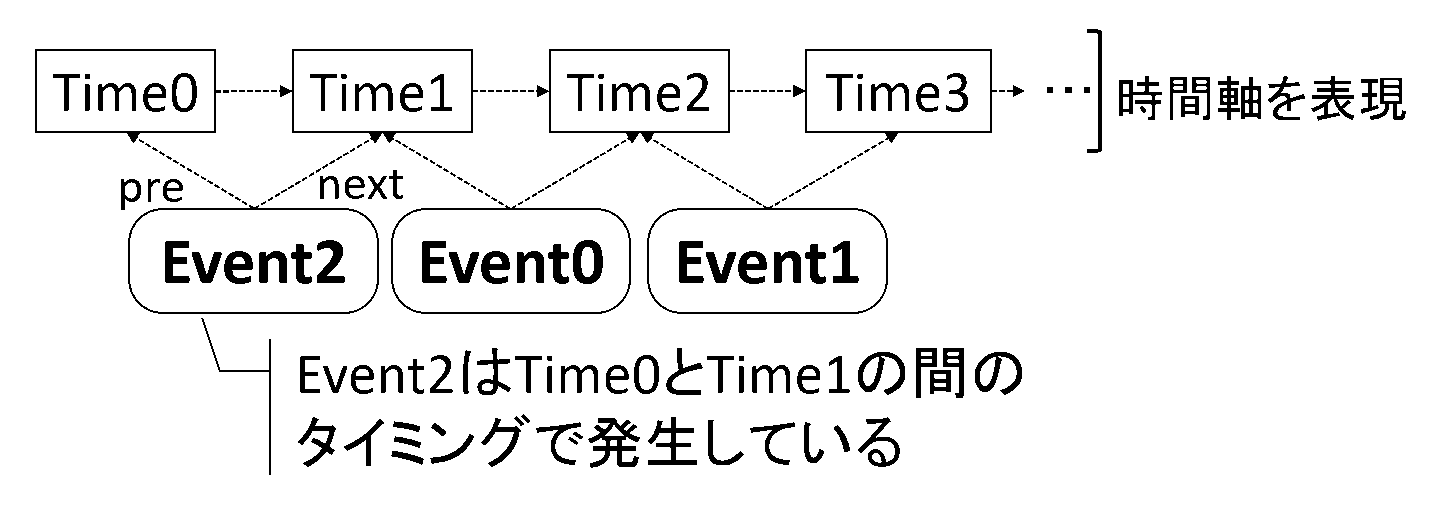
\includegraphics[width=400pt]{./fig/based-model-temporal-logic.eps}
\caption{基礎モデルにおける時間軸とイベントの対応}
\label{fig:based-model-temporal-logic}
\end{figure}
\color{black}

\section{Cookieを包括するモデル}
\subsection{モデルの特徴}
Ryckらによって提案されたウェブセキュリティモデル\cite{cookie-model}(以下
、Cookieモデルとする)は、Akhaweらの基礎モデル(\ref{sec:based-model}節参照)を基にCookieの要素を追加したものである。

\subsection{Cookieモデルの能力}
\color{red}
Cookieモデルは、拡張元である基礎モデルの能力(\ref{sec:based-model-power}節参照)がベースとなっている。
基本的に基礎モデルにおいて包括されている項目に関して変更はないが、Cookieを導入したモデルであるため、ウェブセキュリティモデルの三要素の一つである「対象のシステムの構造と動作」にCookieの動作が包括される。
また、基礎モデルの「安全性要件」に文章上の変更はないが、Security Invariantsにおいて「ウェブの各要素が仕様通りに動作している」ことが求められており、この内容にCookieの動作が追加される。
\color{black}

\subsection{Cookieモデルにおける時相論理の実装}
\color{red}
基礎モデルでは、時相論理はリクエストやレスポンスといったイベントの発生順序を表現するために用いられている。
Cookieモデルではこれに加えて、リクエストとレスポンス間でのCookieの状態変化を表現するために時相論理を用いている。
Cookieに対しての時相論理はCode\ref{code:cookie-model-temporal-logic}に示すコードで実装される。
\begin{lstlisting}[caption=Cookieに対する時相論理, label=code:cookie-model-temporal-logic]
sig CSState {
	dst: Origin,
	cookies: set Cookie
}

sig CSStateHTTPTransaction extends HTTPTransaction {
	beforeState: CSState,
	afterState: CSState
}{
	beforeState.dst = afterState.dst
	afterState.cookies = beforeState.cookies + (resp.headers & SetCookieHeader).thecookie
	
	beforeState.dst = req.host
}
\end{lstlisting}
このCookieに関する時相論理は、基礎モデルにおけるCode\ref{code:based-model-httptransaction}を利用して表現されている。
6~14行目で定義しているCSStateHTTPTransactionは基礎モデルのHTTPTransactionを継承しているクラスであり、対応するリクエストとレスポンス間のCookieの状態変化を表すことができる。
また、1~4行目で定義されているCSStateは、ある時点でのCookieの状態を表現するクラスであり、CSStateHTTPTransactionはリクエスト、レスポンス時それぞれのCSStateを持つ。
Cookieはブラウザでのみ使用される要素であるため、これらのCSStateはそのトランザクションのリクエストの送信元のクライアントのCookieの状態を表す。
%この二つのCSStateの違いを見ることで、あるトランザクションにおけるCookieの変化を捉えることが可能となっている(図\ref{fig:cookie-model-transaction})。
この二つのCSStateの違いを見ることで、あるトランザクションにおけるCookieの変化を捉えることが可能となっている(図挿入予定)。

%\begin{figure}[htb]
%\centering
%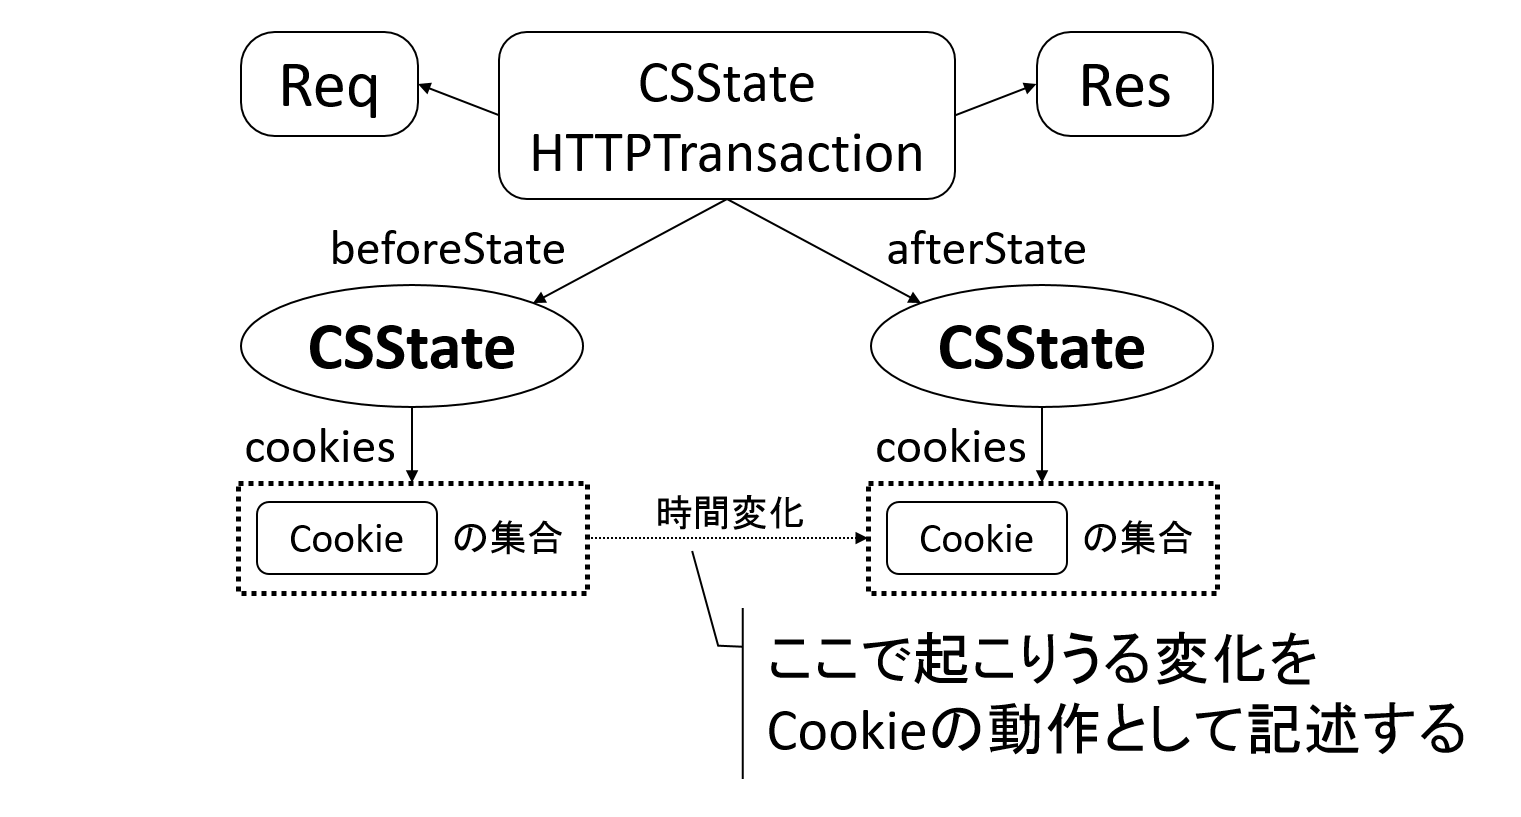
\includegraphics[width=400pt]{./fig/cookie-model-transaction.eps}
%\caption{CookieモデルにおけるCookieの時間変化の表現}
%\label{fig:cookie-model-transaction}
%\end{figure}

\color{black}

\section{既存モデルにおける不足点}
\color{red}
\color{black}

\end{document}

\documentclass[12pt,a4paper]{jbook}
\usepackage{mm-thesis}
\usepackage[dvipdfmx]{graphicx}
\usepackage{cite}
\usepackage{comment}
\usepackage{docmute}
\usepackage{color}
\usepackage{moreverb}
\usepackage{listings}
\usepackage{ascmac}
%\usepackage{amsmath}
%\usepackage{amsthm}
%\usepackage{amsfonts}

\lstset{
	%枠外での自動改行
 	breaklines = true,
 	%標準の書体
 	basicstyle = {\small},
 	%枠 "t"は上に線を記載, "T"は上に二重線を記載
	%他オプション:leftline,topline,bottomline,lines,single,shadowbox
 	frame = TB,
 	%タブの大きさ
 	tabsize = 2,
 	%キャプションの場所("tb"ならば上下両方に記載)
 	captionpos = t,
 	%行番号の位置
 	numbers = left,
 	%自動改行後のインデント量(デフォルトでは20[pt])	
 	breakindent = 30pt,
	%左右の位置調整 	
 	xleftmargin=30pt,
 	xrightmargin=30pt,
	%プログラム言語(複数の言語に対応,C,C++も可)
 	%language = Python, 	
 	%背景色と透過度
 	%backgroundcolor={\color[gray]{.90}},
 	%コメントの書体
 	%commentstyle = {\itshape \color[cmyk]{1,0.4,1,0}},
 	%関数名等の色の設定
 	%classoffset = 0,
 	%キーワード(int, ifなど)の書体
 	%keywordstyle = {\bfseries \color[cmyk]{0,1,0,0}},
 	%表示する文字の書体
 	%stringstyle = {\ttfamily \color[rgb]{0,0,1}},
 	%frameまでの間隔(行番号とプログラムの間)
 	%framesep = 5pt,
 	%行番号の間隔
 	%stepnumber = 1,
	%行番号の書体
 	%numberstyle = \tiny,
}
\renewcommand{\lstlistingname}{Code}
\begin{document}
\newpage

\chapter{提案モデル}
\color{red}
この章では、ウェブの様々な要素に利用可能なAlloyでの時相論理の記述法と、その応用例としてキャッシュを実装したウェブセキュリティモデルを提案する。
\color{black}

\section{汎用的な時相論理のAlloy上の記述法の提案}
\label{sec:ProposedModel-TemporalLogic}
\color{red}
前述の\ref{sec:existing-models-problems}節における既存モデルの時相論理の表現能力の問題点は、「時間軸全体を通して状態変化を追うことができない」ことである。
そもそも、既存モデルが同一のTransaction間の状態変化のみの表現能力となっているのは、状態を表すクラス(CookieモデルにけるCSStateクラス)間の時間軸上での順序の表現を、ツールの機能を利用しない論理式で実現することが難しいためである。
したがって、状態を表すクラス間の時間軸上の関係性を表現できる述語が必要となる。
また、CookieモデルにおけるCSStateクラスはCookieの状態を表現するためのクラスであり、CSStateのみに利用できる述語では今後の他のウェブの要素に利用できない。
以上より、様々なウェブの要素の状態を表現するための汎用的なクラスを定義し、そのクラスに利用可能な述語を作成する。

また、時間軸全体を通して状態変化を表現するためには必要となる述語を考える。
まず、ある状態からその直前の状態を判定できれば、「前後の二状態で起こりうる変化」を表現可能になる。
これに加えて状態遷移の初期状態を判定できれば、「初期状態にかかる条件(初期条件)」を表現可能になる。
これら二つの表現能力を組み合わせることで、帰納的に時間軸全体で起こりうる状態変化を表現可能となる。
したがって、これらの表現能力を実装するため、以下の述語を作成する。
\begin{itemize}
\item Transactionの関係に関わらず、直前にあたる状態を判定する述語
\item 初期状態を判定する述語
\end{itemize}

また、本記述法を用いる上で基礎モデルでの時間軸の表現(\ref{sec:based-model-temporal-logic}節参照)を一部変更している。
その変更点についても以降で述べる。

\subsubsection{時間軸の表現の変更}
基礎モデル\cite{based-model}においては、時間軸を表すTimeクラスにネットワーク上で発生するレスポンスやリクエストを表すEventクラスが関連付けられている。
これらのクラス間の関係性は、「ある時点Time0とTime1の間でEvent0が発生した」といった内容を表現できるというものであり、二つのTimeクラスのインスタンスで一つのイベントの時刻を表現できる。

しかし、本提案モデルではEventクラスに加えて、ある時点におけるウェブの要素の状態を表すStateクラスも時間軸に関連付けられる。
ここで、二つのTimeクラスのインスタンスで一つのイベントの時刻を表現するという既存モデルの関係性を維持すると、導入する述語の論理式が複雑となり実装が困難となる。
したがって、本提案モデルでは図\ref{fig:ProposedModel-TimeClass}に示す、一つのTimeクラスのインスタンスでイベントの時刻を表現できる記述法に変更する。

\begin{figure}[htb]
\centering
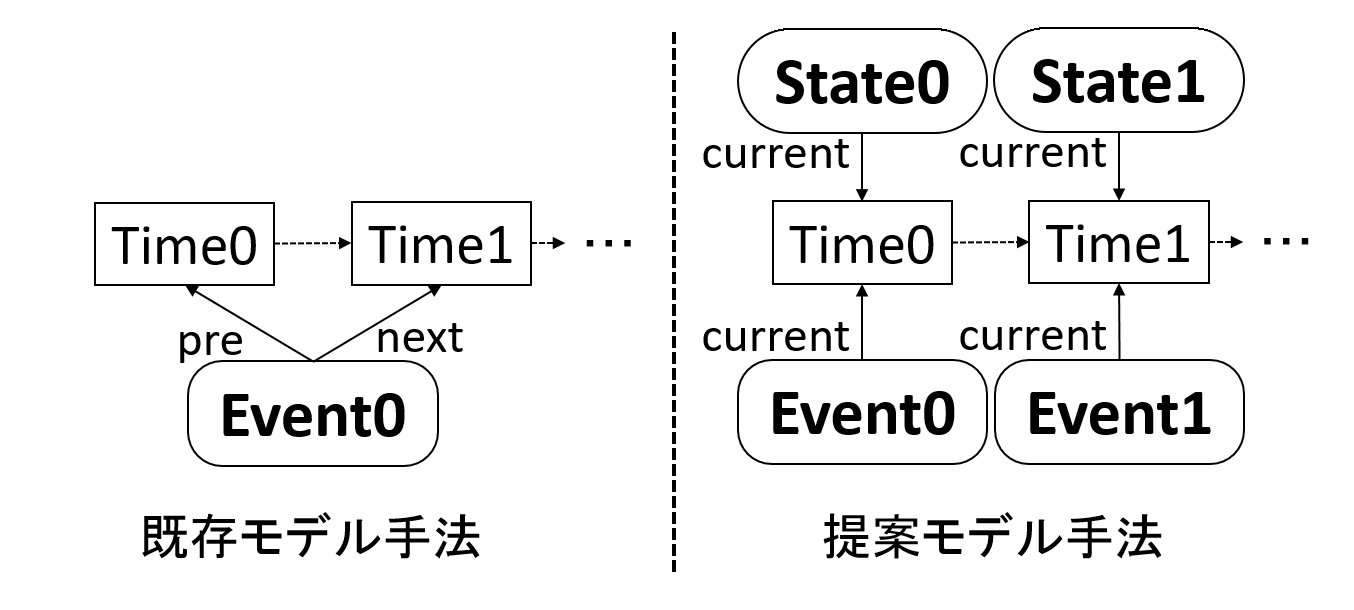
\includegraphics[width=450pt]{./fig/ProposedModel-TimeClass.eps}
\caption{提案モデルにおける時間軸とイベントの関係}
\label{fig:ProposedModel-TimeClass}
\end{figure}

この記述の変更によって、二つの既存モデルそれぞれにおける時相論理の表現能力に変更はない。
そもそも、基礎モデルで二つのTimeクラスのインスタンスを利用する関係性とした理由は、今後の拡張において「リクエストやレスポンスといったイベントが同時刻で発生しない」という基礎モデルの制限を無くすことを想定したためである。
本提案モデルにおいてもこの制限事項は継承しているが、一つのTimeクラスのインスタンスによる表現としたとしても、同じTimeクラスのインスタンスとの関係を持つEventクラスのインスタンスが複数存在することを許容することで今後の拡張は可能である。
つまり、この変更によって既存モデルの表現能力と拡張性を妨げない。

\subsubsection{状態を表現する汎用クラス}
導入する汎用クラスとしてCode\ref{code:StateClass}に示すStateクラスを定義する。
flowはStateクラス同士を接続し状態の遷移を、currentはその状態となり得る時刻を表す。
また、その他の項目としてEqItem、DifItemクラスをStateクラスの変数としている。
\begin{lstlisting}[caption=Stateクラス, label=code:StateClass]
abstract sig State{
	flow: set State,
	eq: one EqItem,
	dif: one DifItem,
	current: set Time
}
abstract sig EqItem{}
abstract sig DifItem{}
sig StateTransaction extends HTTPTransaction{
	beforeState: set State,
	afterState: set State
}
\end{lstlisting}

まず、EqItemは同一の状態遷移上で変化しない要素(以下、「一致要素」とする)を表すクラスである。
一致要素は複数のStateが存在する場合に、いずれのStateが同一の遷移であるのかを判定するために必要である。
例えばStateが三つ存在している場合を考えると、図\ref{fig:ProposedModel-3StateFlow}に挙げられるように複数の遷移のパターンが考えられる。
ここで、EqItemをStateごとに比較をすることで、同一のEqItemを持つStateを同一の遷移に存在すると判定することができる。
図\ref{fig:ProposedModel-3StateFlow}を例にとると、三状態が同一の遷移に存在する場合にはState0,1,2のEqItemがすべて同じとなる。
一方で、三状態が同一の遷移に存在しない場合にはState0,2のEqItemが同じであり、State1のEqItemはそれと異なる。

\begin{figure}[htb]
\centering
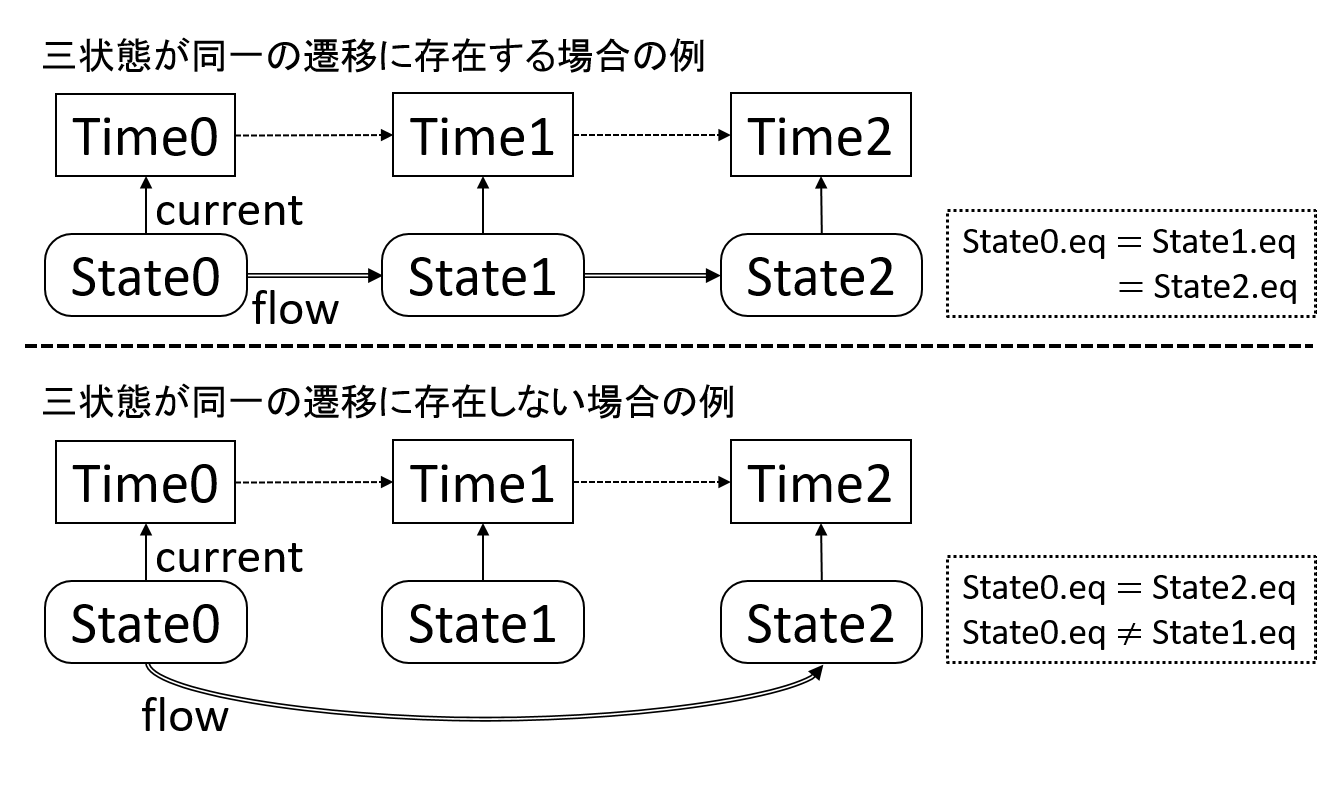
\includegraphics[width=400pt]{./fig/ProposedModel-3StateFlow.eps}
\caption{3Stateによる遷移の例}
\label{fig:ProposedModel-3StateFlow}
\end{figure}

また、DifItemは状態遷移において変化する要素(以下、「変化要素」とする)を表すクラスである。
状態変化をモデルで表現した際に捉えたい項目をDifItemに記述する。

最後に、これらのStateはCookieモデルと同様にHTTPTransactionに関連付けることで、レスポンスとリクエスト時の状態を表す。
したがって、HTTPTransactionを継承しStateクラスを持つStateTransactionをCode\ref{code:StateClass}の9-12行目で定義している。

このStateクラスを利用してウェブの要素の状態遷移を考えるには、State、EqItem、DifItemクラスを継承するその要素専用のクラスを定義する。
また、その要素について一致要素と変化要素を明らかにしておき、継承後のクラスに記述する。
以下のCode\ref{code:CookieClass}はCookieモデルを基にしたCookieへの応用例である。
2,3行目に記すように、Stateを継承するクラスではeqとdifもまた、EqItem、DifItemを継承する専用のクラスに含まれるように条件を記述する。
Cookieモデルでは、一致要素がクライアント、変化要素がCookieの集合となっている。
これは、各クライアント毎にでCookieの保存が行われているため、状態遷移の上でクライアントは変更されないためである。
また、変化要素は変化を捉えたい要素である、クライアント内で保存されているCookieを表現している。
\begin{lstlisting}[caption=Cookieへの応用例, label=code:CookieClass]
sig CookieState extends State{}{
	eq in CookieEqItem
	dif in CookieDifItem
}
sig CookieEqItem extends EqItem{
	client: one HTTPClient
}
sig CookieDifItem extends DifItem{
	cookie: set Cookie
}
\end{lstlisting}

\subsubsection{直前状態を判定する述語}
上記のStateクラスに対して、状態遷移上で直前となる状態を判定する述語JustBeforeStateを利用できる(Code\ref{code:JustBeforeState}参照)。
このJustBeforeStateは三つの引数を要する。
そのうちの二つはStateクラスでありそれぞれpre、postと表す。
述語JustBeforeStateはpreがpostの直前の状態であるか考える。
しかし、postが複数の時刻を持つ場合があり、この場合には二つのStateの入力では複数の組み合わせで真となる。
そこで、postの時刻を指定するため、StateTransactionを引数に追加する(これをstrとする)。
これにより、与えられたトランザクションに含まれるpostの時刻に限定して、その時刻においてpreが直前であるか判定でき、真となる組み合わせが一意に定まる。
\begin{lstlisting}[caption=状態遷移において直前の状態を判定する述語, label=code:JustBeforeState]
pred JustBeforeState[pre:State, post:State, str:StateTransaction]{
	pre.eq = post.eq
	post in str.(beforeState + afterState)

	some t,t':Time |
		{
			t in pre.current
			t' in str.(request + response + re_res).current
			t' in str.request.current implies post in str.beforeState
			t' in str.(response + re_res).current implies post in str.afterState
			t' in t.next.*next

			all s:State, t'':Time |
				(s.eq = pre.eq and t'' in s.current) implies
						(t in t''.*next) or (t'' in t'.*next)
		}
}
\end{lstlisting}
この述語JustBeforeStateが真となる条件は以下の三つに分割でき、引数がすべてを満たす場合に述語JustBeforeStateも真となる。
\begin{itemize}
\item preとpostの一致要素が同一であること(2行目)
\item postがstrのbeforeState、afterStateのいずれかに属していること(3行目)
\item preの時刻とpostのstrにおける時刻の間に、一致要素が同一の他の状態が存在しないこと(5-16行目)
\end{itemize}

%\subsubsection{初期状態を判定する述語}
%Stateクラスに対して利用可能な、もう一方の述語は初期状態を判定する述語FirstStateである(Code\ref{code:FirstState}参照)。
%\begin{lstlisting}[caption=状態遷移において初期状態を判定する述語, label=code:FirstState]
%pred FirstState[s:State]{
%	all s':State |
%		s.eq = s'.eq implies
%			s'.current in s.current.*next	//s => s'
%}
%\end{lstlisting}


\section{提案記述法を用いたキャッシュの実装}
\section{中継者の実装}
\color{black}
\section{提案モデルの制限事項}

\end{document}

\documentclass[12pt,a4paper]{jbook}
\usepackage{mm-thesis}
\usepackage[dvipdfmx]{graphicx}
\usepackage{cite}
\usepackage{comment}
\usepackage{docmute}
\usepackage{color}
\usepackage{moreverb}
\usepackage{listings}
\usepackage{ascmac}
%\usepackage{amsmath}
%\usepackage{amsthm}
%\usepackage{amsfonts}

\lstset{
	%枠外での自動改行
 	breaklines = true,
 	%標準の書体
 	basicstyle = {\small},
 	%枠 "t"は上に線を記載, "T"は上に二重線を記載
	%他オプション:leftline,topline,bottomline,lines,single,shadowbox
 	frame = TB,
 	%タブの大きさ
 	tabsize = 2,
 	%キャプションの場所("tb"ならば上下両方に記載)
 	captionpos = t,
 	%行番号の位置
 	numbers = left,
 	%自動改行後のインデント量(デフォルトでは20[pt])	
 	breakindent = 30pt,
	%左右の位置調整 	
 	xleftmargin=30pt,
 	xrightmargin=30pt,
	%プログラム言語(複数の言語に対応,C,C++も可)
 	%language = Python, 	
 	%背景色と透過度
 	%backgroundcolor={\color[gray]{.90}},
 	%コメントの書体
 	%commentstyle = {\itshape \color[cmyk]{1,0.4,1,0}},
 	%関数名等の色の設定
 	%classoffset = 0,
 	%キーワード(int, ifなど)の書体
 	%keywordstyle = {\bfseries \color[cmyk]{0,1,0,0}},
 	%表示する文字の書体
 	%stringstyle = {\ttfamily \color[rgb]{0,0,1}},
 	%frameまでの間隔(行番号とプログラムの間)
 	%framesep = 5pt,
 	%行番号の間隔
 	%stepnumber = 1,
	%行番号の書体
 	%numberstyle = \tiny,
}
\renewcommand{\lstlistingname}{Code}
\begin{document}
\newpage

\chapter{事例研究}
本章では、複数の具体的な事例を取り上げ、提案モデルの実装の正しさを確認する。

\section{キャッシュの基本動作}
本節では、提案モデルでのキャッシュの実装の正しさを確認する。
提案モデルにおいて、キャッシュは主に格納、再利用、検証の三つの動作を行う。
それぞれについて、実行ツールAlloy Analyzerの実行結果を確認する。

\subsection{レスポンスの格納}
レスポンスの格納動作を確認するため、実行結果からレスポンスの格納を伴う動作を含む結果を抽出する。
ここでは簡単のため、最も単純な二者間における通信で生じるレスポンスの格納を対象とし、Code\ref{code:test_store}を用いて出力を得る。
Code\ref{code:test_store}はクライアントとサーバの二者間における一組のリクエストとレスポンスの通信において、格納レスポンス集合に要素が存在するキャッシュの状態が存在する結果を出力するものである。

\begin{lstlisting}[caption=レスポンスの格納, label=code:test_store]
run test_store{
	#HTTPClient = 1
	#HTTPServer = 1
	#HTTPRequest = 1
	#HTTPResponse = 1
	some CacheState.dif.store
} for 2
\end{lstlisting}

得られる出力結果を整理し、図\ref{fig:TestStore}に示す。
図\ref{fig:TestStore}には、PrivateCache0を持つBrowser0とServer0間の、Request0とResponse0のトランザクションにおけるキャッシュの状態変化が示されている。
最初、リクエスト時にはキャッシュの状態はCacheState0で示されており、CacheState0の変化要素を表すCacheDifItem0のstoreが空集合である。
しかし、レスポンス時には状態はCacheState1に変化しており、対応するCacheDifItem1がResponse0にstoreを指している。
以上より、図\ref{fig:TestStore}はあるトランザクションにおいて、レスポンスがブラウザキャッシュに格納されている状態を表しており、レスポンスの格納が表現可能であることが確認できる。

\begin{figure}[htb]
\centering
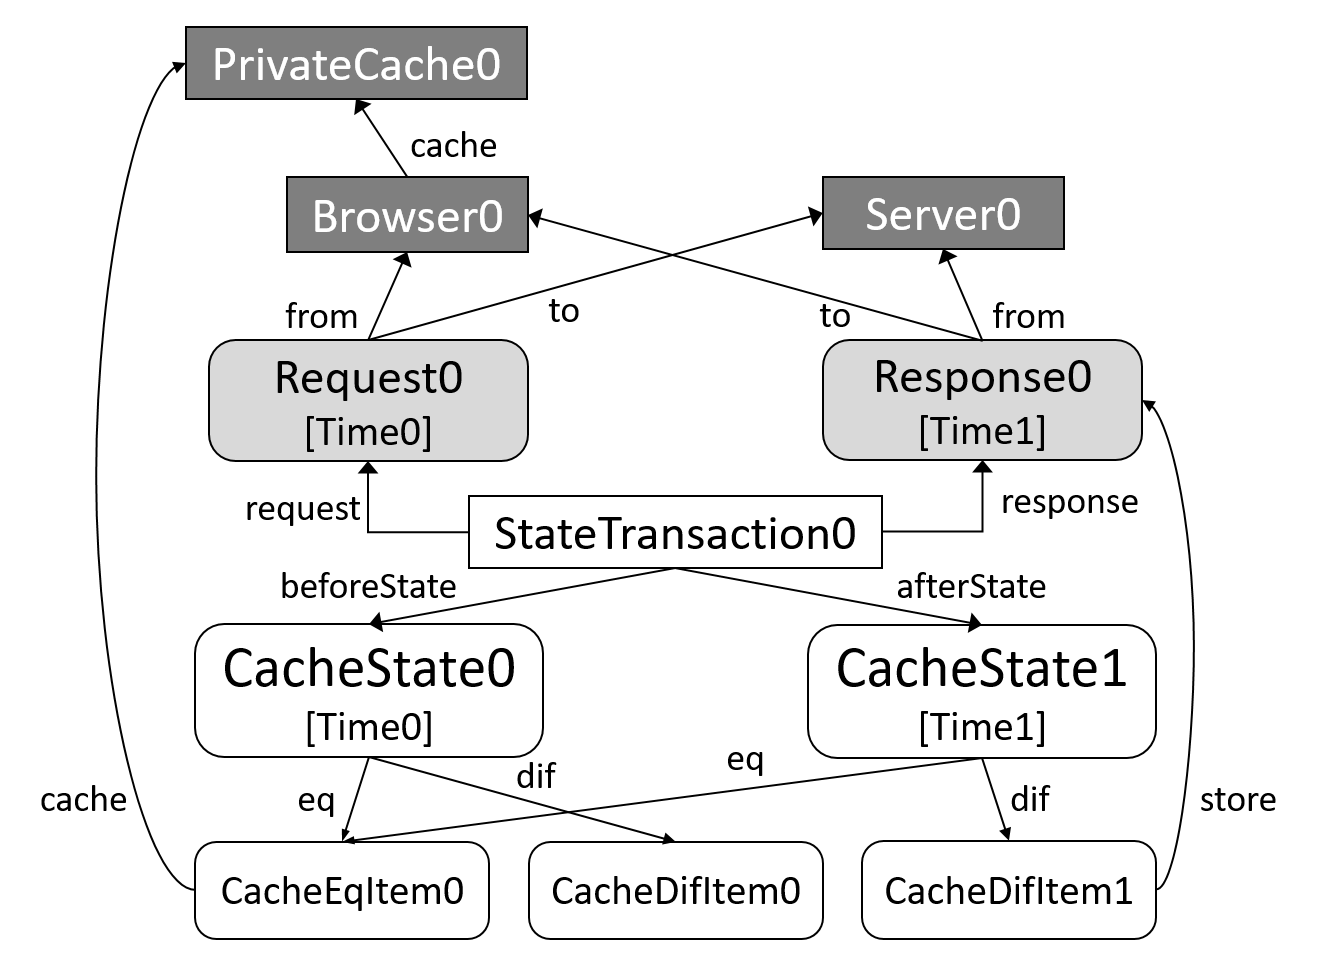
\includegraphics[width=450pt]{./fig/TestStore.eps}
\caption{レスポンスを格納する状態の一例}
\label{fig:TestStore}
\end{figure}

\subsection{格納レスポンスの再利用}
レスポンスの再利用動作を確認するため、実行結果からレスポンスの再利用を伴う動作を含む結果を抽出する。
ここでは簡単のため、最も単純な二者間における通信で生じるレスポンスの再利用を対象とし、Code\ref{code:test_reuse}を用いて出力を得る。
Code\ref{code:test_reuse}はクライアントとサーバの二者間における二組の通信において、一度レスポンスの再利用が発生している結果を出力するものである。

\begin{lstlisting}[caption=格納レスポンスの再利用, label=code:test_reuse]
run test_reuse{
	#HTTPClient = 1
	#HTTPServer = 1
	#Cache = 1

	#HTTPRequest = 2
	#HTTPResponse = 1
	#CacheReuse = 1
} for 4
\end{lstlisting}

得られる出力結果をスペースの都合上一部簡略化し、図\ref{fig:TestReuse}に示す。
図\ref{fig:TestReuse}はあるキャッシュを持つブラウザとサーバ間で、同様のURIに対してリクエストが二回送信された状態を表している。
ここで、StateTransaction0では図\ref{fig:TestStore}と同様、ブラウザキャッシュにResponse0を格納している。
StateTransaction1では、この格納レスポンスを再利用するイベントCacheReuse0が発生している。
以上より、図\ref{fig:TestReuse}に示す出力結果から、再利用を伴う動作が表現可能であることが確認できる。

\begin{figure}[htb]
\centering
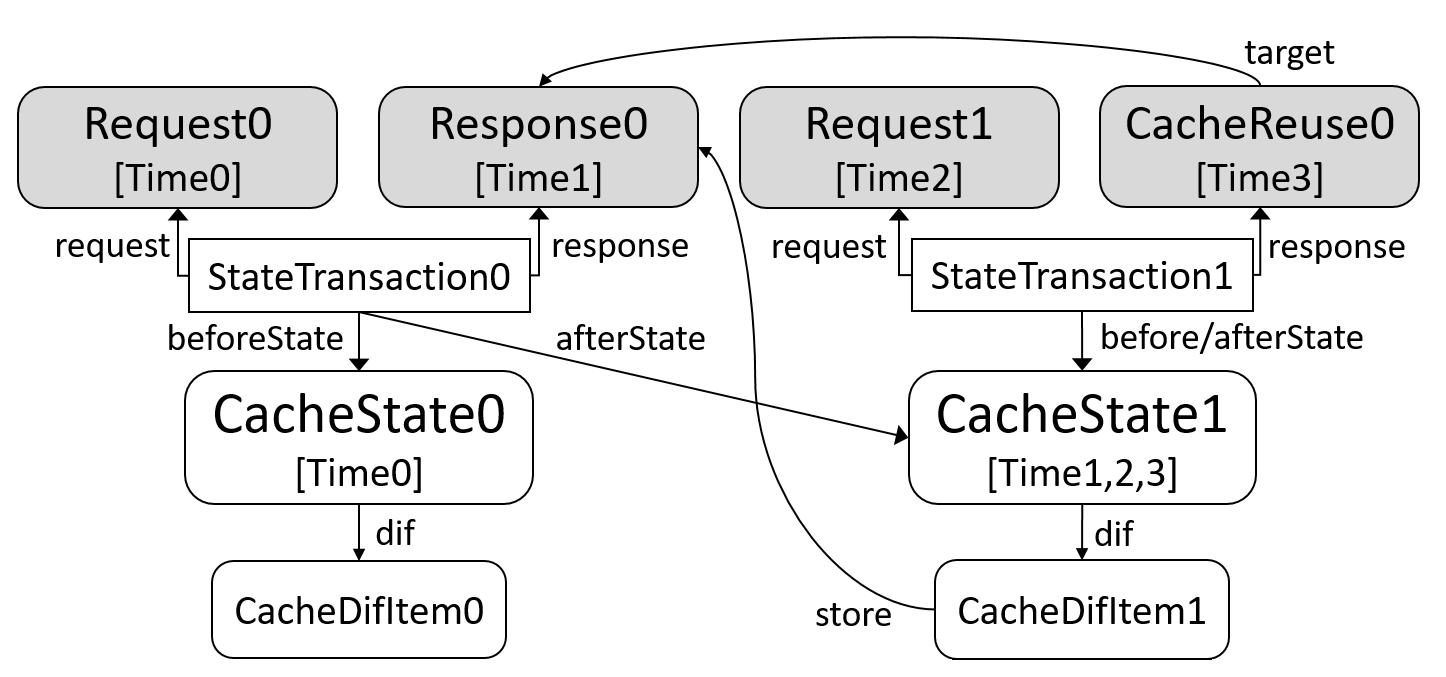
\includegraphics[width=450pt]{./fig/TestReuse.eps}
\caption{格納レスポンスを再利用する状態の一例}
\label{fig:TestReuse}
\end{figure}

\subsection{格納レスポンスの検証}
レスポンスの検証動作を確認するため、実行結果からレスポンスの検証を伴う動作を含む結果を抽出する。
ここでは簡単のため、最も単純な二者間における通信で生じるレスポンスの検証を対象とし、Code\ref{code:test_verification}を用いて出力を得る。
Code\ref{code:test_verification}はクライアントとサーバの二者間における三組の通信のうち、検証が行われた通信が存在する結果を出力する。
ここで検証が行われたかの判定は、\ref{sec:CacheVerification}節で述べたCode\ref{code:checkVerification}を利用している。

\begin{lstlisting}[caption=格納レスポンスの検証, label=code:test_verification]
run test_verification{
	#HTTPClient = 1
	#HTTPServer = 1
	#HTTPIntermediary = 0
	#Cache = 1
	#PrivateCache = 1

	some str:StateTransaction | checkVerification[str]
} for 6
\end{lstlisting}

得られる出力結果をスペースの都合上一部簡略化し、図\ref{fig:TestVerification}に示す。
図\ref{fig:TestVerification}はあるキャッシュを持つブラウザとサーバ間での、三つの通信(StateTransaction0,1,2)が存在している状態を表しており、このうちStateTransaction2が検証を行っている通信である。
まず、StateTransaction0では図\ref{fig:TestStore}と同様、ブラウザキャッシュにResponse0を格納している。
次に、Request2に対してブラウザキャッシュ内に格納されているResponse0を再利用するため、StateTransaction2で検証動作を行っている。
ここで、格納レスポンスのResponse0にはEtagHeaderが含まれているため、検証に用いる条件付きリクエストであるRequest1にはIfNoneMatchHeaderが含まれている。
また、検証結果となるResponse1は再利用可能であることを示す304の状態コードとなっているため、Response0はそのまま再利用可能であることが示されている。
以上を踏まえて、StateTransaction1ではResponse0をそのまま再利用している。

\begin{figure}[htb]
\centering
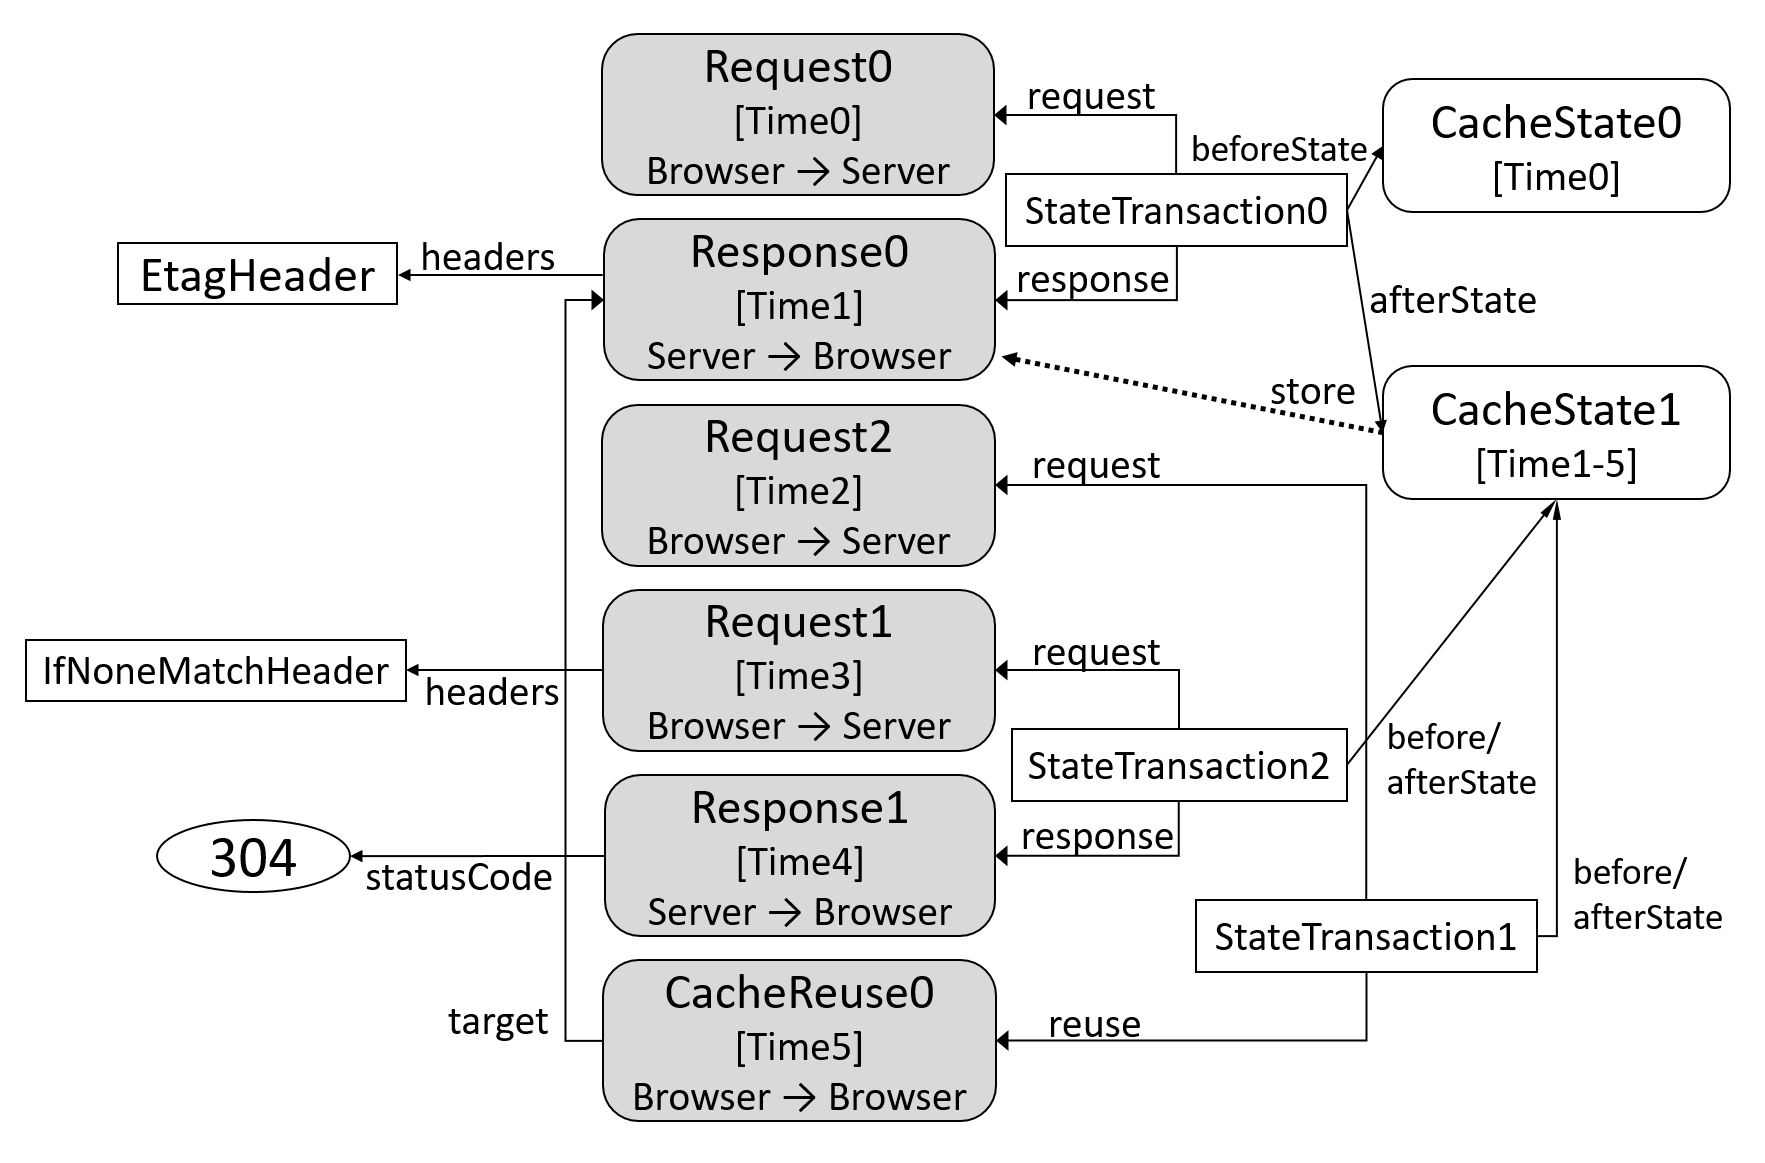
\includegraphics[width=450pt]{./fig/TestVerification.eps}
\caption{格納レスポンスの検証が含まれる状態の一例}
\label{fig:TestVerification}
\end{figure}

\section{中継者の基本動作}
中継者の動作を確認するため、実行結果から中継者の動作を伴う動作を含む結果を抽出する。
ここでは簡単のため、最も単純なクライアント、中継者、サーバが各一つずつ存在する経路において、中継者を経由する通信を対象としCode\ref{code:test_reuse}を用いて出力を得る。

\begin{lstlisting}[caption=中継者の動作, label=code:test_intermediary]
run test_intermediary{
	#HTTPRequest = 2
	#HTTPResponse = 2

	#HTTPClient = 1
	#HTTPServer = 1
	#HTTPIntermediary = 1

	all i:HTTPIntermediary | i in Alice.servers

	one req:HTTPRequest | req.to in HTTPIntermediary
	one req:HTTPRequest | req.to in HTTPServer
} for 4
\end{lstlisting}

得られる出力結果をスペースの都合上一部簡略化し、図\ref{fig:TestIntermediary}に示す。
図\ref{fig:TestIntermediary}で、HTTPTransaction0はブラウザと中継者間の通信、HTTPTransaction1は中継者とサーバ間の通信を表す。
中継者は自身に届けられたリクエストやレスポンスを回送する役割を持ち、このHTTPTransaction0,1が中継者による回送を表している。
以上より、中継者の動作が表現可能であることが確認できる。

\begin{figure}[htb]
\centering
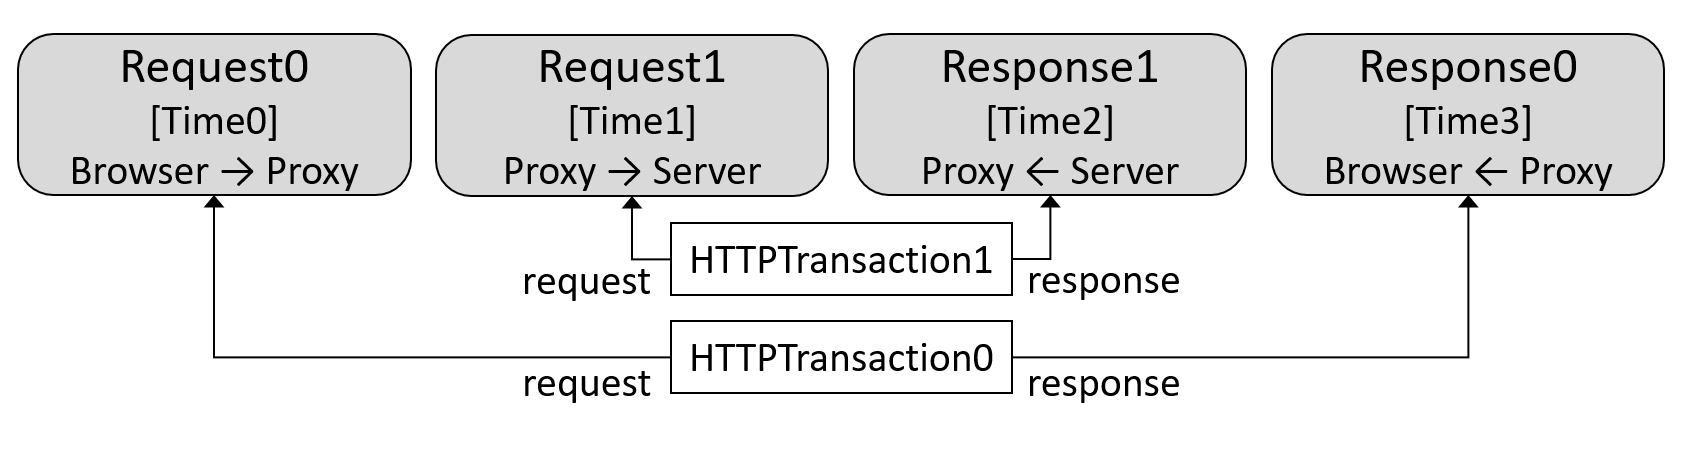
\includegraphics[width=450pt]{./fig/TestIntermediary.eps}
\caption{中継者の動作を含む状態の一例}
\label{fig:TestIntermediary}
\end{figure}

\section{Same-origin Browser Cache Poisoning Attack}
\label{sec:same-origin-bcp}
本節では、提案モデルでSame-origin Browser Cache Poisoning Attack\cite{bcpattack}(以下、Same-origin BCP攻撃とする)が表現可能であるかを確認する。

\subsection{攻撃の概要とフロー}
Same-origin BCP攻撃は、攻撃者の持つ中継者が攻撃対象であるブラウザとサーバの経路上に入り込む「中間者攻撃」の一種である。
本攻撃の目的は対象のブラウザ、攻撃者の任意の動作を実行させることを目的とする。
また、本攻撃の特徴は、攻撃者による通信経路の割り込みが一度であるにも関わらず、そのレスポンスを再利用するたびにブラウザが悪影響を受けるという影響の持続性にある。

攻撃全体のフローを図\ref{fig:SameBCP_flow}に示す。
本攻撃による攻撃者のふるまいは、通信経路上において本来ブラウザが受け取るはずのレスポンスの内容に改ざん(図\ref{fig:SameBCP_flow}内の「4.改ざんレスポンス」)を行い、ブラウザが保有するキャッシュに改ざんレスポンスを格納させることである。
この際の攻撃者による改ざん内容は以下の二点である。
\begin{itemize}
\item レスポンスのヘッダをブラウザキャッシュによるレスポンスの格納や再利用を誘発するよう改ざんする。例えば、有効期限の延長や、検証動作なしの再利用の許可が挙げられる
\item レスポンスのボディに攻撃者に実行させたい任意の動作を記述する
\end{itemize}
また、ブラウザに悪影響が及ぶのは「5.改ざんレスポンスをキャッシュに格納」時と「6.同じファイルの利用時に改ざんレスポンスを再利用」時である。
また、6は改ざんレスポンスがキャッシュ内に格納されている間、何度も繰り返される可能性がある。

\begin{figure}[htb]
\centering
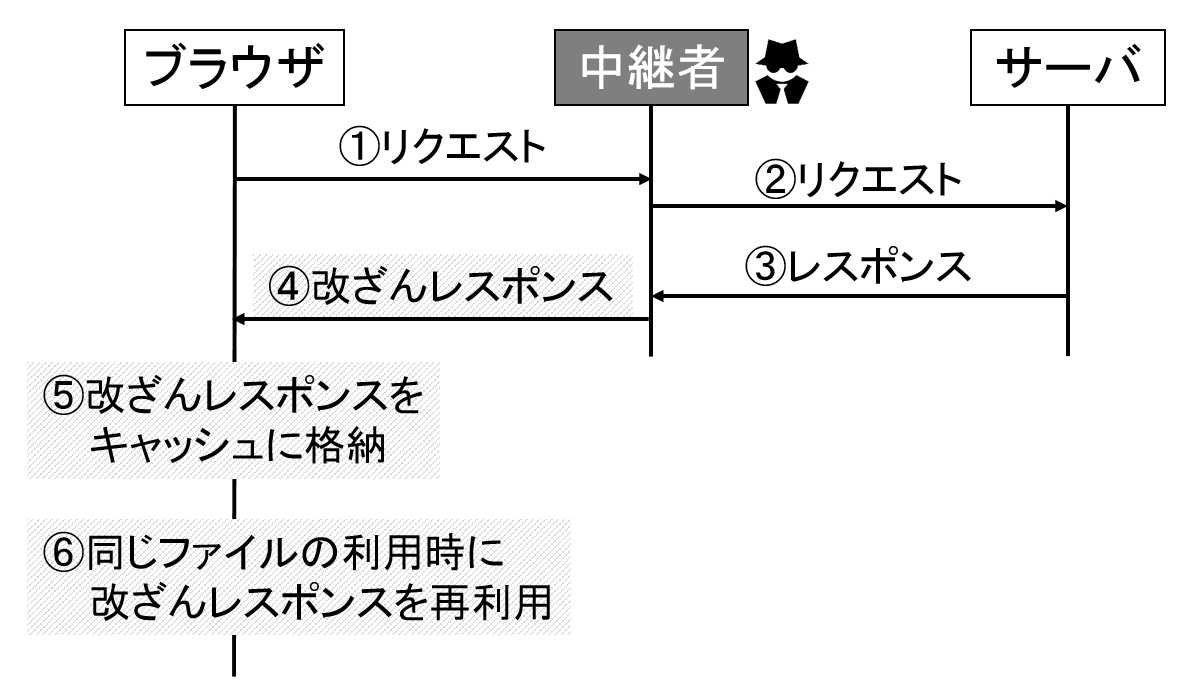
\includegraphics[width=400pt]{./fig/SameBCP_flow.eps}
\caption{Same-origin Browser Cache Poisoning Attackの攻撃フロー}
\label{fig:SameBCP_flow}
\end{figure}

\subsection{提案モデルによる出力}
提案モデルによるSame-origin BCP攻撃の表現を確認するため、実行結果から図\ref{fig:SameBCP_flow}のフローを含む結果を抽出する。
抽出にはCode\ref{code:Same_origin_BCP}を用いる。
実行結果として、図\ref{fig:SameBCP_flow}に従ったフローと、攻撃者によるヘッダとボディの改ざんを含む状態が得られた。
このことから、提案モデルがSame-origin BCP攻撃を表現できることを確認した。

\begin{lstlisting}[caption=Same-origin BCP攻撃の表現, label=code:Same_origin_BCP]
run Same_origin_BCP{
	#HTTPClient = 1
	#HTTPServer = 1
	#HTTPIntermediary = 1
	#PrivateCache = 1
	#PublicCache = 0

	#HTTPRequest = 3
	#HTTPResponse = 2
	#CacheReuse = 1

	#Principal = 3
	#Alice = 2

	some tr,tr',tr'':HTTPTransaction | {
		tr'.request.current in tr.request.current.*next
		tr.response.current in tr'.response.current.*next
		tr''.request.current in tr.response.current.*next
		some tr''.re_res

		tr.request.from in HTTPClient
		tr.request.to in HTTPIntermediary

		tr'.request.from in HTTPIntermediary
		tr'.request.to in HTTPServer

		tr''.request.from in HTTPClient

		tr.response.body != tr'.response.body
	}

	some c:HTTPClient | c in Alice.httpClients
	some s:HTTPServer | s in Alice.servers
	no i:HTTPIntermediary | i in Alice.servers
} for 6
\end{lstlisting}

\section{Cross-site Request Forgeries Attack}
本節では、提案モデルでCross-site Request Forgeries Attack\cite{cookie-model}(以下、CSRF攻撃とする)が表現可能であるかを確認する。

\subsection{攻撃の概要とフロー}
CSRF攻撃は攻撃対象となるサーバと攻撃者が保有するサーバ、そして一般的なブラウザの三者間で実現される攻撃である。
本攻撃の目標は、攻撃対象であるサーバに対して、攻撃者が許されていない動作を実行させることである。

攻撃全体のフローを図\ref{fig:CSRF_flow}に示す。
本攻撃における攻撃者のふるまいは、自身が保有するサーバにアクセスしてきたブラウザが攻撃対象であるサーバへのリクエスト(図\ref{fig:SameBCP_flow}内の「3.リクエスト」)を送信を誘発するようにレスポンス(図\ref{fig:SameBCP_flow}内の「2.レスポンス」)を返すことである。
また、この攻撃者からのレスポンスの内容によって、ブラウザから送信されるリクエストも操作される。

\begin{figure}[htb]
\centering
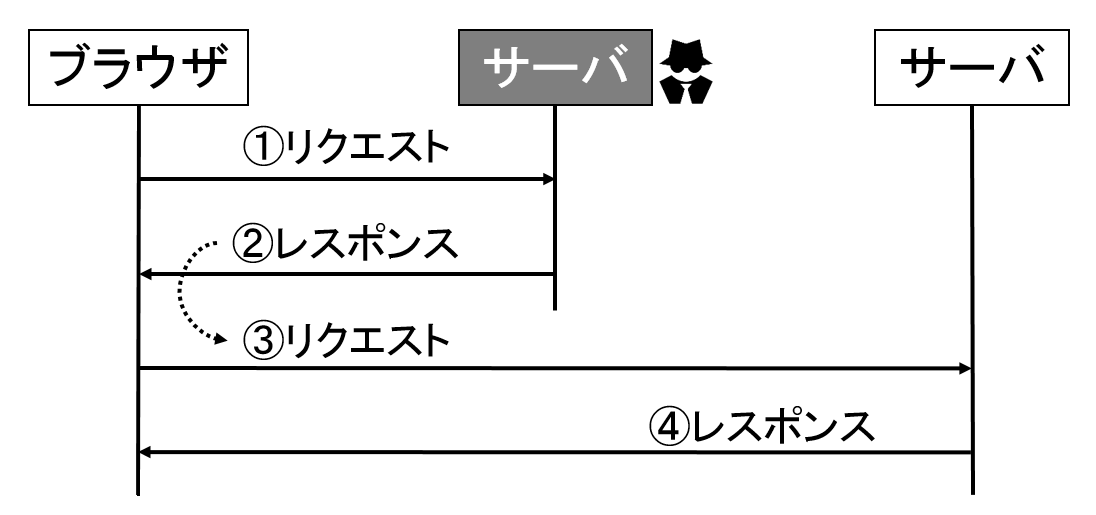
\includegraphics[width=400pt]{./fig/CSRF_flow.eps}
\caption{Cross-site Request Forgeries Attackの攻撃フロー}
\label{fig:CSRF_flow}
\end{figure}

\subsection{提案モデルによる出力}
提案モデルによるCSRF攻撃の表現を確認するため、実行結果から図\ref{fig:CSRF_flow}のフローを含む結果を抽出する。
抽出にはCode\ref{code:CSRF}を用い、その実行結果として図\ref{fig:CSRF_flow}に示す攻撃フローを含む結果が出力された。
スペースの都合上、これを一部簡略化し図\ref{fig:CSRF_alloy}に示す。
図\ref{fig:CSRF_alloy}において、Server0が攻撃者のサーバ、Server1が攻撃対象のサーバを表している。
また、HTTPTransaction0はBrowserがServer0にアクセスした通信を、HTTPTransaction1はそれに誘発されたBrowserとServer1の通信を表している。
HTTPTransaction1はHTTPTransaction0にcauseの関係を持ち、これがHTTPTransaction0に誘発されていることを示している。
以上のことから、CSRF攻撃を含む出力結果が得られているため、提案モデルがCSRF攻撃を表現できることを確認した。

\begin{lstlisting}[caption=CSRF攻撃の表現, label=code:CSRF]
run CSRF{
	#HTTPRequest = 2
	#HTTPResponse = 2

	#HTTPClient = 1
	#HTTPServer = 2
	#HTTPIntermediary = 0

	#Principal = 3
	#Alice = 2

	all p:Principal |
		one c:HTTPConformist |
			c in p.(servers + httpClients)
	all b:Browser | b in Alice.httpClients

	one tr1,tr2:HTTPTransaction|{
		tr2.request.current in tr1.response.current.*next

		tr1.request.to !in Alice.servers
		tr2.request.to in Alice.servers

		tr2.cause = tr1

		tr1.request.uri != tr2.request.uri
	}
} for 4
\end{lstlisting}

\begin{figure}[htb]
\centering
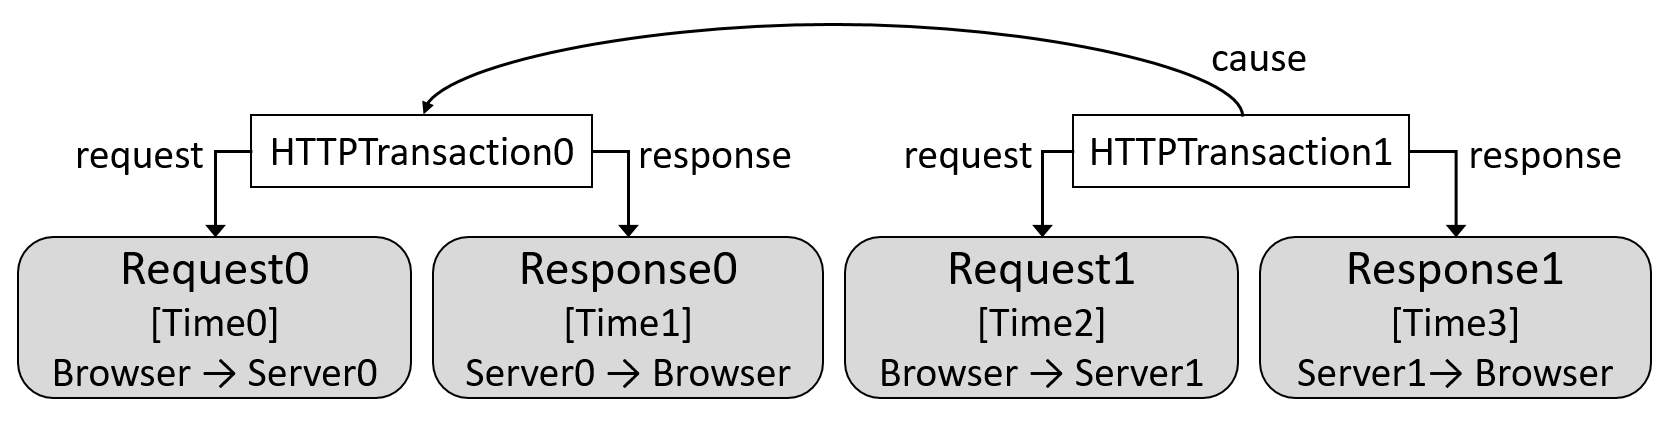
\includegraphics[width=450pt]{./fig/CSRF_alloy.eps}
\caption{CSRF攻撃のフローを含む状態の一例}
\label{fig:CSRF_alloy}
\end{figure}

\section{Cross-origin Browser Cache Poisoning Attack}
本節では、提案モデルでCross-origin Browser Cache Poisoning Attack\cite{bcpattack}(以下、Cross-origin BCP攻撃とする)が表現可能であるかを確認する。

\subsection{攻撃の概要とフロー}
Cross-origin BCP攻撃は、\ref{sec:same-origin-bcp}節で述べたSame-origin BCP攻撃と同様に「中間者攻撃」一種である。
Same-origin BCP攻撃に比べ、改ざんレスポンスの再利用の頻度を高めることができる。
これは、Cross-origin BCP攻撃では、任意のファイルのレスポンスに改ざんを行うことができることに起因する。
これにより、一つのサイトだけでなく多くのサイトに共通して利用されるようなファイル(cssやjsファイルなど)を改ざんの対象とすることができる。
これに対して、\ref{sec:same-origin-bcp}節で記述のSame-origin BCP攻撃は、攻撃者がファイルを指定することはできず、通信に介入した際に偶然行われていた通信のみを改ざん可能な対象とする。

Cross-origin BCP攻撃は図\ref{fig:CrossBCP_flow}に示す攻撃フローで実現される。
ここで、図\ref{fig:CrossBCP_flow}内での「5.リクエスト」以降は、Same-origin BCP攻撃と同一のフローである。
また、それ以前のフローについては、CSRFのフローと役割が類似している。
まず最初に、攻撃者は「1.リクエスト」の通信に介入し、レスポンスの改ざんを行う。
ここにおける改ざんは、実際に改ざんを試みるファイルに対しての「5.リクエスト」の誘発を目的とする。
例えば、「A.css」という多くのページで共通して使用されるファイルが存在する場合、「3.レスポンス」の内容にA.cssを利用するよう追記することで、A.cssに対する「5.リクエスト」を誘発することができる。
したがって、図\ref{fig:CrossBCP_flow}のフローによって、攻撃者が指定する任意のファイルの改ざんを行い、そのレスポンスをブラウザキャッシュに格納させることができる。
また、このフローの成功後はサーバ1,2に無関係な通信であったとしても、改ざんレスポンスに記述されているファイルを利用する際には再利用が発生し、ブラウザは悪影響を受ける。

\begin{figure}[htb]
\centering
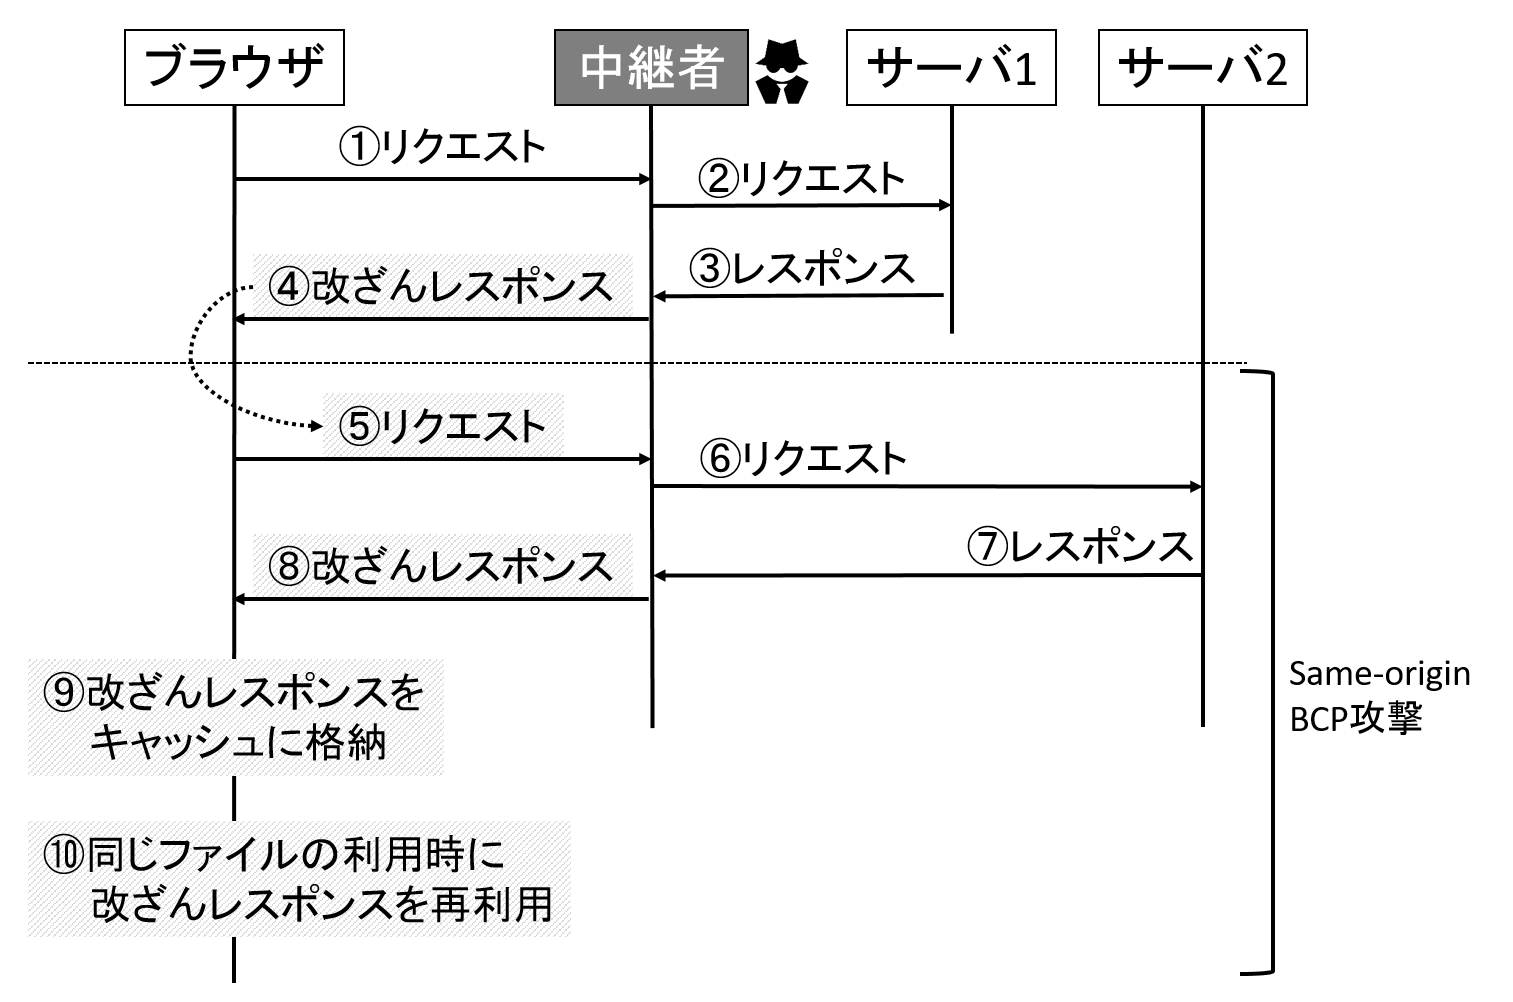
\includegraphics[width=450pt]{./fig/CrossBCP_flow.eps}
\caption{Cross-origin Browser Cache Poisoning Attackの攻撃フロー}
\label{fig:CrossBCP_flow}
\end{figure}

\subsection{提案モデルによる出力}
提案モデルによるCSRF攻撃の表現を確認するため、実行結果から図\ref{fig:CrossBCP_flow}を含む結果を抽出する。
結果として、図\ref{fig:CrossBCP_flow}に存在する五つの通信を表現された状態を出力した。
このことから、提案モデルがCross-origin BCP攻撃を表現できることを確認した。
また、スペースの都合上、実行コードは巻末付録Code\ref{code:Cross_origin_BCP}に記載する。

\section{Web Cache Deception Attack}
本節では、提案モデルでWeb Cache Deception Attack\cite{WCD}(以下、WCD攻撃とする)が表現可能であるかを確認する。

\subsection{攻撃の概要とフロー}
WCD攻撃は攻撃対象となるサーバと中継者、二つのブラウザで成り立つ攻撃である。
攻撃者はこれらのうち一つのブラウザを所有し、本来、攻撃者がサーバから得ることのできないファイルを取得することが目的である。

WCD攻撃は図\ref{fig:WCD_flow}に示す攻撃フローで実現される。
まず、攻撃者にアクセス権の無いファイルに対して、正当なユーザに中継者を経由してアクセスさせる。
この際に、そのレスポンス(図\ref{fig:WCD_flow}内の「3.レスポンス」)が中継者のキャッシュに格納された場合、攻撃者はその中継者を含む経路でそのファイルに対するリクエスト(図\ref{fig:WCD_flow}内の「5.リクエスト」)を送信することで、そのファイルを取得することができる(図\ref{fig:WCD_flow}内の「6.格納レスポンスの再利用」)。

\begin{figure}[htb]
\centering
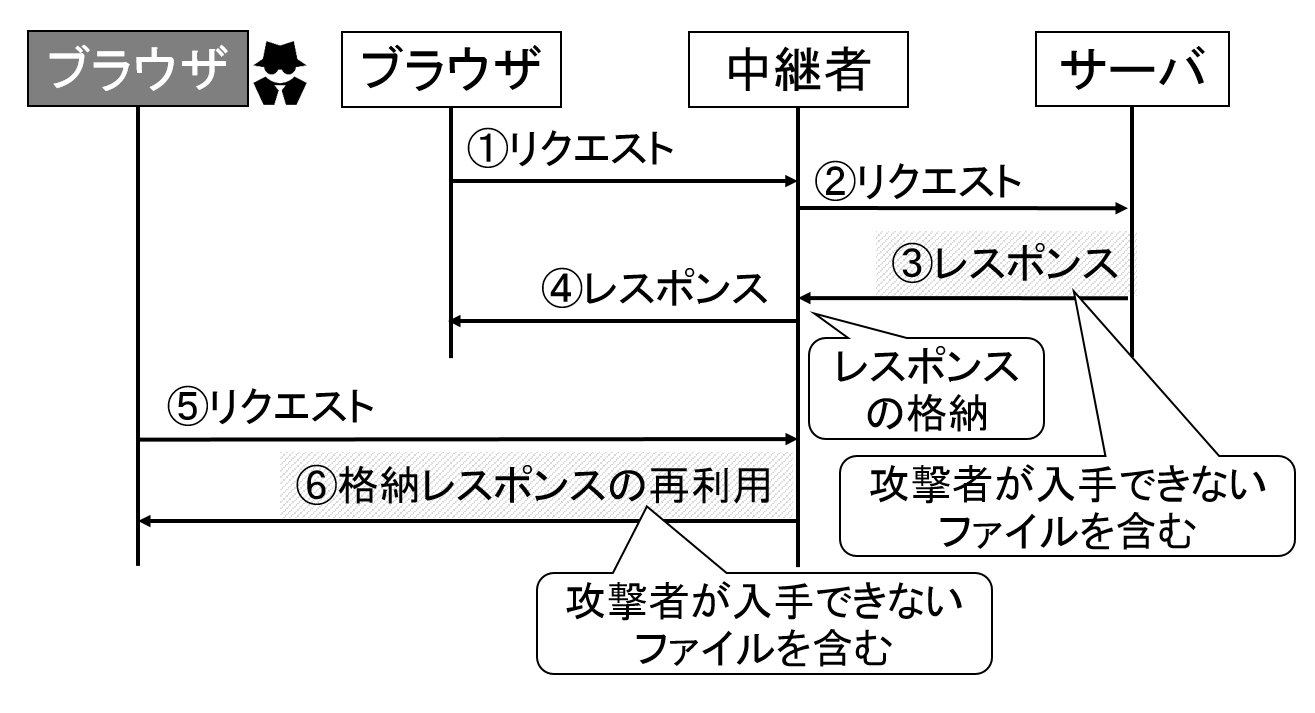
\includegraphics[width=450pt]{./fig/WCD_flow.eps}
\caption{Web Cache Deception Attackの攻撃フロー}
\label{fig:WCD_flow}
\end{figure}

\subsection{提案モデルによる出力}
提案モデルによるWCD攻撃の表現を確認するため、実行結果から図\ref{fig:WCD_flow}のフローを含む結果を抽出する。
抽出にはCode\ref{code:WCD}を用い、その実行結果として図\ref{fig:WCD_flow}に示す攻撃フローを含む結果が出力された。
スペースの都合上、これを一部簡略化し図\ref{fig:WCD_alloy}に示す。
図\ref{fig:WCD_alloy}において、図\ref{fig:WCD_flow}の「1.リクエスト」と「2.リクエスト」の通信はStateTransaction0,1でそれぞれ表されている。
ここで、Response1のボディにはTokenが付与されており、これが攻撃者がアクセス権を持たないファイルを示している。
このResponse1は、その発生時刻Time2で中継者のキャッシュに保存され、攻撃者による通信StateTransaction2において再利用されている。
従って、この出力結果は攻撃者が本来権限を持たないファイルを中継者のキャッシュによる再利用を用いて取得していることを表している。
以上のことから、WCD攻撃を含む出力結果が得られているため、提案モデルがWCD攻撃を表現できることを確認した。

\begin{lstlisting}[caption=WCD攻撃の表現, label=code:WCD]
run Web_Cache_Deception{
	#HTTPRequest = 3
	#HTTPResponse = 2
	#CacheReuse = 1

	#HTTPClient = 2
	#HTTPServer = 1
	#HTTPProxy = 1
	#Cache = 1

	#Principal = 4
	#Alice = 3

	all c:Cache | c in HTTPProxy.cache

	all p:Principal |
		one c:HTTPConformist |
			c in p.(servers + httpClients)
	all i:HTTPProxy | i in Alice.servers
	all s:HTTPServer | s in Alice.servers

	one tr1,tr2,tr3:HTTPTransaction |{
		tr1.request.from in Alice.httpClients
		tr1.request.to in HTTPProxy

		tr2.request.from in HTTPProxy
		tr2.request.to in HTTPServer

		(tr3.request.from !in Alice.httpClients and tr3.request.from in HTTPClient)
		tr3.request.to in HTTPProxy

		one tr3.re_res
	}
} for 6
\end{lstlisting}

\begin{figure}[htb]
\centering
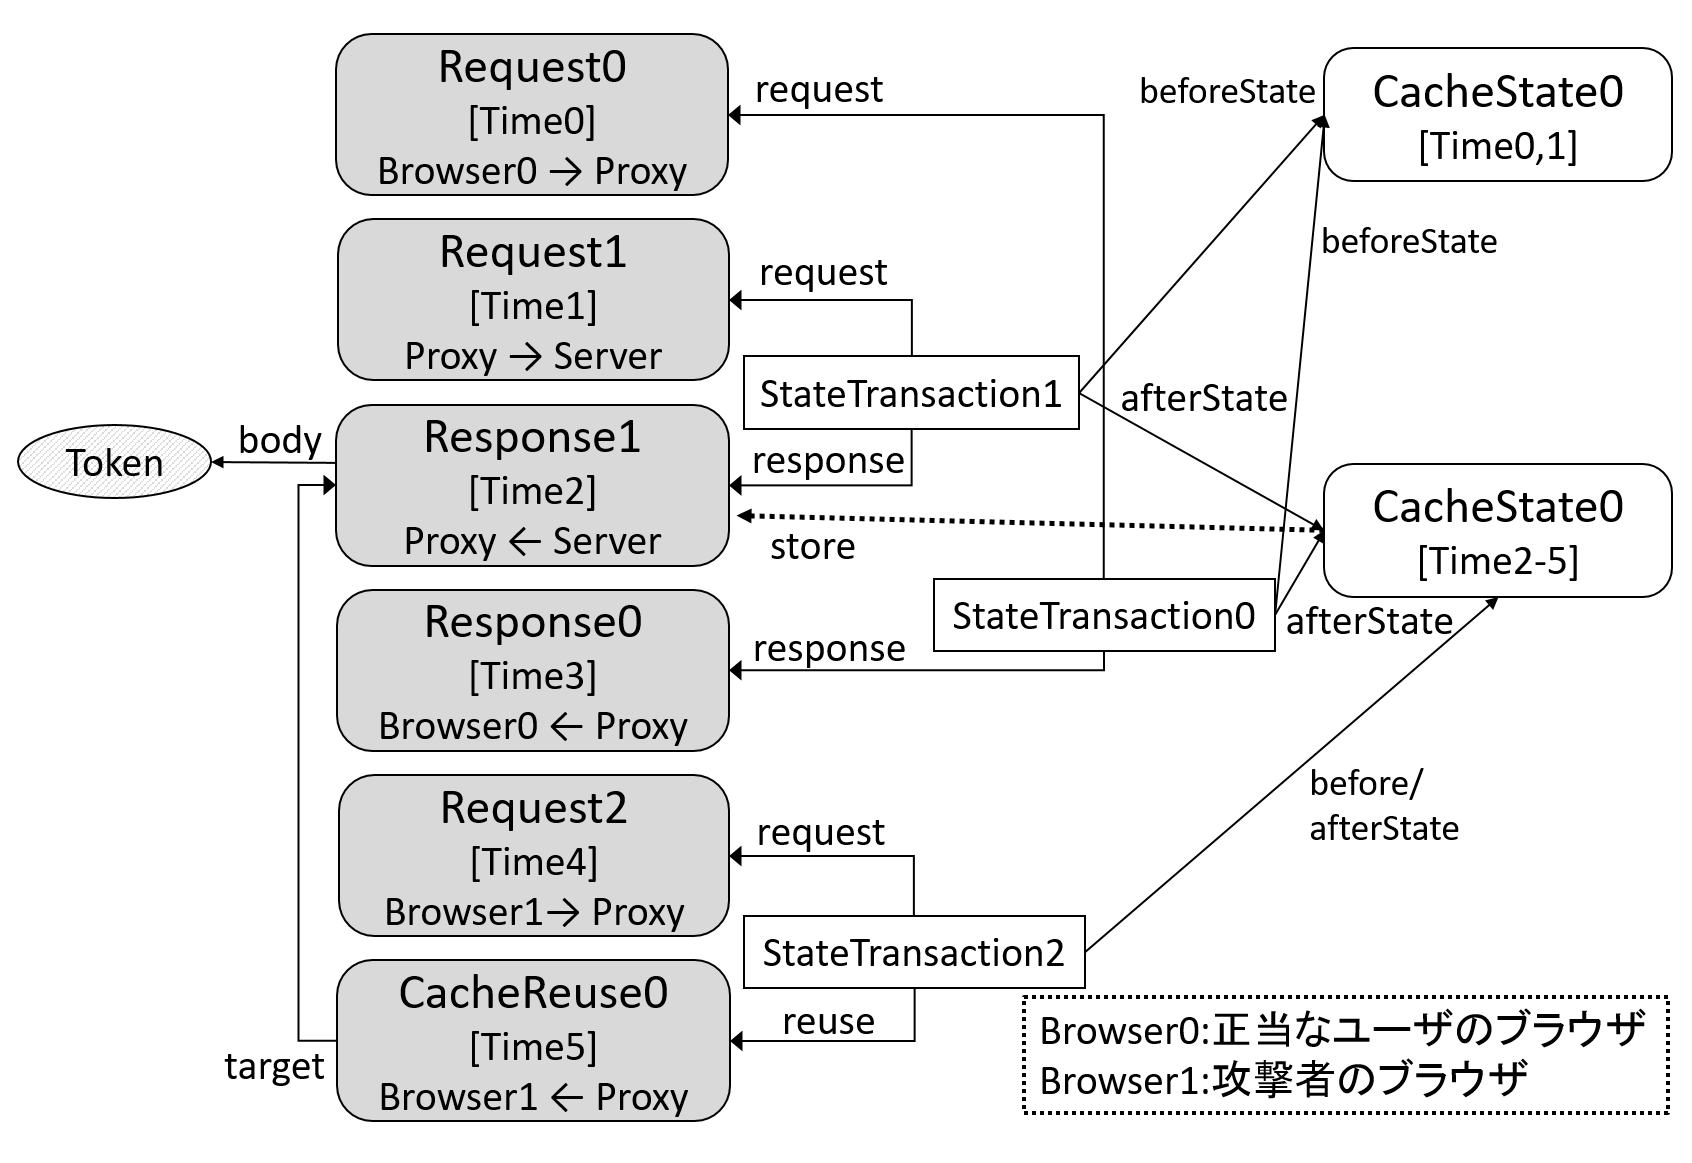
\includegraphics[width=450pt]{./fig/WCD_alloy.eps}
\caption{WCD攻撃のフローを含む状態の一例}
\label{fig:WCD_alloy}
\end{figure}

\end{document}

\documentclass[12pt,a4paper]{jbook}
\usepackage{mm-thesis}
\usepackage[dvipdfmx]{graphicx}
\usepackage{cite}
\usepackage{comment}
\usepackage{docmute}
\usepackage{color}
\usepackage{moreverb}
\usepackage{listings}
\usepackage{ascmac}
%\usepackage{amsmath}
%\usepackage{amsthm}
%\usepackage{amsfonts}

\lstset{
	%枠外での自動改行
 	breaklines = true,
 	%標準の書体
 	basicstyle = {\small},
 	%枠 "t"は上に線を記載, "T"は上に二重線を記載
	%他オプション:leftline,topline,bottomline,lines,single,shadowbox
 	frame = TB,
 	%タブの大きさ
 	tabsize = 2,
 	%キャプションの場所("tb"ならば上下両方に記載)
 	captionpos = t,
 	%行番号の位置
 	numbers = left,
 	%自動改行後のインデント量(デフォルトでは20[pt])	
 	breakindent = 30pt,
	%左右の位置調整 	
 	xleftmargin=30pt,
 	xrightmargin=30pt,
	%プログラム言語(複数の言語に対応,C,C++も可)
 	%language = Python, 	
 	%背景色と透過度
 	%backgroundcolor={\color[gray]{.90}},
 	%コメントの書体
 	%commentstyle = {\itshape \color[cmyk]{1,0.4,1,0}},
 	%関数名等の色の設定
 	%classoffset = 0,
 	%キーワード(int, ifなど)の書体
 	%keywordstyle = {\bfseries \color[cmyk]{0,1,0,0}},
 	%表示する文字の書体
 	%stringstyle = {\ttfamily \color[rgb]{0,0,1}},
 	%frameまでの間隔(行番号とプログラムの間)
 	%framesep = 5pt,
 	%行番号の間隔
 	%stepnumber = 1,
	%行番号の書体
 	%numberstyle = \tiny,
}
\renewcommand{\lstlistingname}{Code}
\begin{document}

\chapter{おわりに}

\end{document}


\acknowledgement
まず,本研究を進める全過程において多大な御指導を賜りました藤原融教授に深く感謝致します.
また,矢内直人助教,岡村真吾招聘准教授に心より御礼申し上げます.
そして,日常の議論を通じて多くのアドバイスや指摘を下さった藤原研究室の皆様ならびに,円滑な研究生活のために諸事務手続きを行って下さった秘書の方々に感謝致します.

\bibliographystyle{junsrt}
\bibliography{list} 

\end{document}


